%!TEX root = ../Report.tex

In this chapter, we discuss the results obtained from the experiments performed using our synthetic test program.

Each section provides the results of the experiments described in the corresponding section in chapter \ref{chapter:experimental_methodology}, which describes each experiment.



\section{Performance Characteristics Investigation}
\label{section:results:performance_characteristics_investigation}

In this section we discuss the results obtained by the performance characteristics investigation. As such, two experiments were performed, each assessing different aspects of the simple synthetic Jacobi stencil code. The first deals with how barrier synchronisation, required for the program to be correct, affects performance, and the second deals with how convergence checks affect performance.



\subsection{Barrier Synchronisation}
\label{section:results:barrier_syncronisation}

In this experiment, we evaluated three options of barriers for the synthetic test program. One using a custom implementation, one using the pthreads implementation, and one using no barrier at all. Without a barrier the program is incorrect, however we include it to get a feel for the performance impact of the barrier, as we expect it to be significant. The results of this can be seen in figure \ref{fig:barrier_sync}.



\begin{figure}[H]
    \begin{center}
        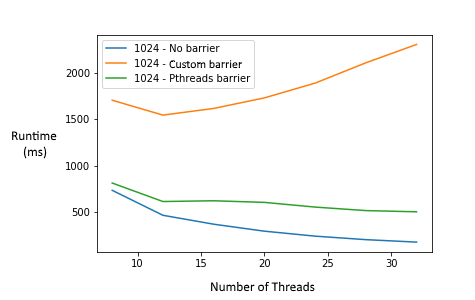
\includegraphics[width=0.85\textwidth]{graphics/performance_characteristics/barrier-1024.png}
        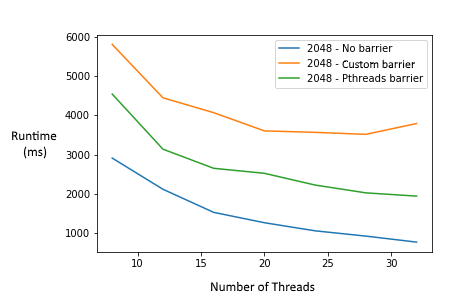
\includegraphics[width=0.85\textwidth]{graphics/performance_characteristics/barrier-2048.png}
    \end{center}
    \caption{A set of graphs which show the runtimes of different barrier options in milliseconds against the number of threads used. The first graph is at grid size 1024, the second at 2048. Run on XXXII, each point is the mean of 100 repeats, with insignificant variance. Computation at each point is the basic jacobi stencil.}
    \label{fig:barrier_sync}
\end{figure}



\begin{figure}[H]
    \centerline{
    \begin{tabular}{||c c||} 
            \hline
            \textbf{num\_runs:} & 101 \\
            \hline
            \textbf{num\_stages:} & 1 \\
            \hline
            \textbf{grid\_size:} & 1024 \\
            \hline
            \textbf{num\_iterations\_0:} & 500 \\
            \hline
            \textbf{set\_pin\_bool\_0:} & 0 \\
            \hline
            \textbf{pinnings\_0:} & - \\
            \hline
            \textbf{kernel\_repeats\_0:} & - \\
            \hline
            \textbf{kernel\_durations\_0:} & - \\
            \hline
            \textbf{kernels:} & - \\
            \hline
            \textbf{num\_workers\_0:} & 8 \\ [1ex] 
            \hline
        \end{tabular}
    }
    \caption{The base config settings used for the barrier synchronisation experiment, the results of which are given in figure \ref{fig:barrier_sync}. Certain settings will change for different tests.}
    \label{fig:barrier_sync_config}
\end{figure}



From figure \ref{fig:barrier_sync}, we can see that using any kind of barrier adds a consistent performance penalty. Also, that our custom barrier implementation performs significantly worse compared to the pthreads implementation. This provides another example of the difficulties of parallel programming, as the custom barrier is an implementation of a standard counter barrier algorithm, whereas the pthreads implementation has had the benefit of rigorous performance tuning over many years.

Another takeaway from these results is that at smaller grid sizes, and with only the basic jacobi work to do (no additional workload,) the barrier synchronisation has a more significant effect on the runtime. Indeed, looking at the case with a grid size of 1024 and 32 threads, the runtime can increase by a factor of 2-8x, depending on the barrier implementation.

After this experiment, we used the pthreads barrier implementation, as this is the version which would be selected by a performance conscience application programmer.



\subsection{Convergence Checks}
\label{section:results:convergence_checks}

In this experiment, we evaluate how the stencil convergence checks affect the performance of the synthetic test program. To this effect, we performed tests at multiple large grid sizes, with and without the convergence checks. All experiments unless otherwise stated include simulated convergence checks, more details can be found in section \ref{section:experimental_methodology:convergence_checks}. The results of these experiments can be seen in figure \ref{fig:convergence_checks}.



\begin{figure}[H]
    \vspace*{-1.5in}
    \begin{center}
        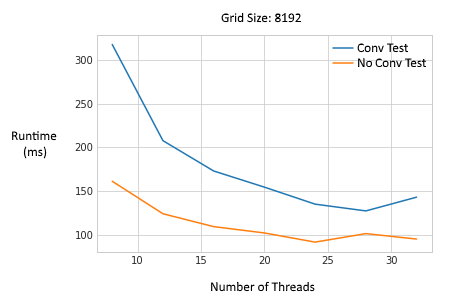
\includegraphics[width=0.85\textwidth]{graphics/performance_characteristics/conv-8192.png}
        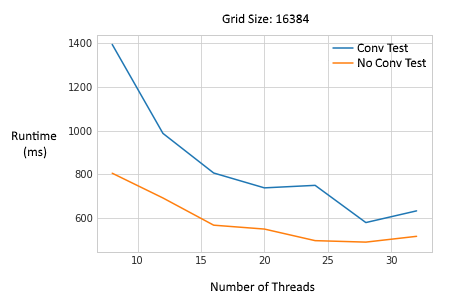
\includegraphics[width=0.85\textwidth]{graphics/performance_characteristics/conv-16384.png}
        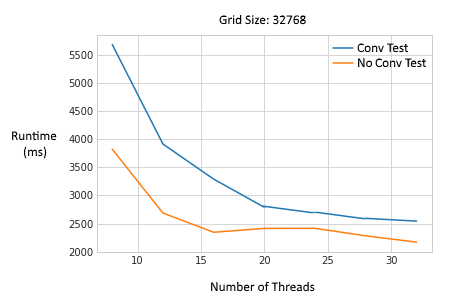
\includegraphics[width=0.85\textwidth]{graphics/performance_characteristics/conv-32768.png}
    \end{center}
    \caption{A set of graphs which demonstrate how the convergence test affects the performance of our synthetic test program. Each graph plots the runtime, in milliseconds, of our synthetic test program, with and without the convergence test, against the number of threads used. The three graphs show the case with a grid size of 8192, 16384, and 32768 respectively. Run on XXXII, each point is the mean of 100 repeats, with insignificant variance. Computation at each point is the basic jacobi stencil.}
    \label{fig:convergence_checks}
\end{figure}



\begin{figure}[H]
    \centerline{
    \begin{tabular}{||c c||} 
            \hline
            \textbf{num\_runs:} & 101 \\
            \hline
            \textbf{num\_stages:} & 1 \\
            \hline
            \textbf{grid\_size:} & 1024 \\
            \hline
            \textbf{num\_iterations\_0:} & 10 \\
            \hline
            \textbf{set\_pin\_bool\_0:} & 0 \\
            \hline
            \textbf{pinnings\_0:} & - \\
            \hline
            \textbf{kernel\_repeats\_0:} & - \\
            \hline
            \textbf{kernel\_durations\_0:} & - \\
            \hline
            \textbf{kernels:} & - \\
            \hline
            \textbf{num\_workers\_0:} & 8 \\ [1ex] 
            \hline
        \end{tabular}
    }
    \caption{The base config settings used for the convergence checks experiment, the results of which are given in figure \ref{fig:convergence_checks}. Certain settings will change for different tests.}
    \label{fig:convergence_checks_config}
\end{figure}



The results presented in figure \ref{fig:convergence_checks} are generally what we would expect. We see that at all grid sizes, the convergence test has a scaling cost, relative to the number of threads. This makes sense as the convergence test can be efficiently partitioned between threads.

We can also see that the convergence test has a significant cost, sometimes doubling the runtime of our synthetic test program. This is using the basic jacobi kernel of summing each point's neighbours however, and as we use more complex kernels, the relative cost will go down.

Additionally, these results show the effect doubling the grid length (with a square grid, so four times as much data.) The runtime seems to scale roughly linearly with regards to the amount of data in the grid, for equivalent numbers of threads, with and without the convergence test. We can see that, in the case with eight threads and no convergence test, at grid size 8192 we have a runtime of approximately 160ms. After quadrupling the amount of data (at gridsize 16384,) we have a runtime of approximately 800ms. After quadrupling again, we have a runtime of approximately 3800ms. These characteristics may change however when we use less predictable workloads.



\section{Finding Interesting Instances}
\label{section:results:finding_interesting_instances}

The purpose of these experiments is to find interesting instances, from a performance perspective, of the basic jacobi stencil. This involves adding a weightier computation kernel to be run at each point in the grid, in addition to the basic jacobi stencil. We would like to identify two or three different types of kernel, which stress different resources of the system.

For each of these, as discussed in section \ref{section:design:interesting_instances}, we want to find one example where adding more threads harms the overall performance, and one example where the program can use as many threads as we can give it. To find such examples, we performed a measured exploration of the ``performance space'' of each kernel, the details of which are as follows:



\subsection{A Range of Computation Kernels}
\label{section:results:a_range_of_computation_kernels}

Our first step was to come up with some different possible kernels. We want kernels which stress different resources, so we decided to create kernels which stress the CPU and the virtual memory. Other resources could also be targeted (e.g. I/O or HDD,) but to keep the number of experiments manageable, we focused on the typically most important resources. 

From there, we have multiple options to create computation kernels, using different functions and methods. We compared the performance characteristics for a variety of kernels, and how they performed with different numbers of threads, and at different grid sizes. The results can be seen in figure \ref{fig:quicktest}.



\begin{figure}[H]
    \vspace*{-1.5in}
    \centerline{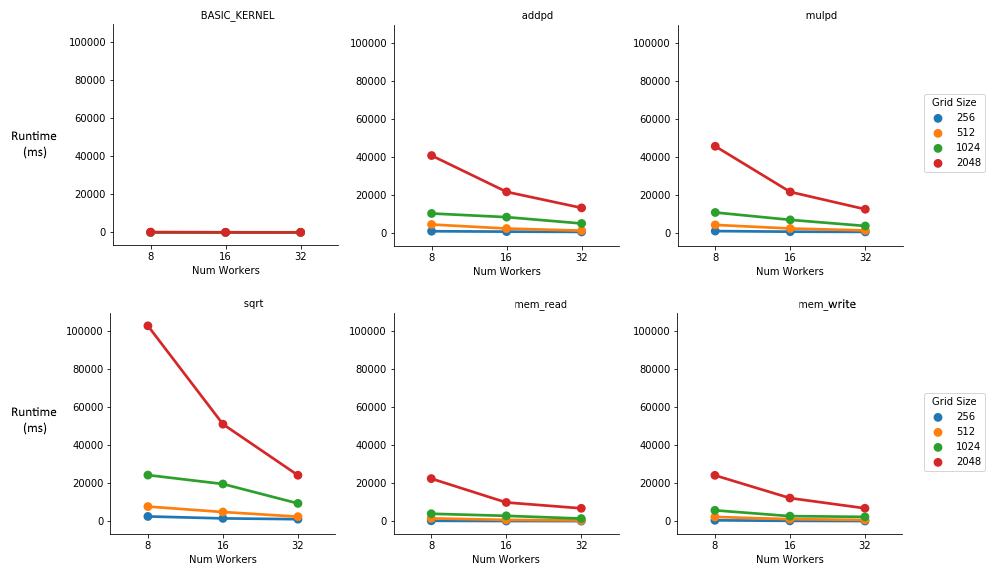
\includegraphics[width=1.5\textwidth]{graphics/interesting_instances/quicktest.png}}
    \captionsetup{singlelinecheck=off}
    \caption[foo bar]{These graphs show the runtimes, in milliseconds, of various computation kernels with various grid sizes, against the number of threads used. Run on XXXII, each point is the mean of 10 repeats, with insignificant variance. We have fewer repeats with these graphs, as these graphs were part of a range whose only purpose was to let us get a feel for the performance characteristics of different kernels, such that we can select appropriate kernels for subsequent experiments. The kernels are as follows:
    \begin{itemize}
        \item \textbf{BASIC\_KERNEL:} This kernel has no additional computation, it is simply the basic jacobi kernel. We include it here for comparison.
        \item\textbf{addpd:} This kernel is designed to stress the CPU using repeated addition operations. Specifically, with the x86 operation ADDPD: Add Packed Double-Precision Floating-Point Values.
        \item \textbf{mulpd:} This kernel is designed to stress the CPU using repeated multiplication operations. Specifically, with the x86 operation MULPD: Multiply Packed Double-Precision Floating-Point Values.
        \item \textbf{sqrt:} This kernel is designed to stress the CPU using repeated sqrt operations. Specifically, using the sqrt() function from the standard math library.
        \item \textbf{mem\_read:} This kernel is designed to stress the VM using repeated memory operations. Specifically, we allocate a portion of memory, and then we step through it, touching (reading) certain values.
        \item \textbf{mem\_write:} This kernel is designed to stress the VM using repeated memory operations. Specifically, we allocate a portion of memory, and then we step through it, writing certain values.
    \end{itemize}}
    \label{fig:quicktest}
\end{figure}



\begin{figure}[H]
    \centerline{
    \begin{tabular}{||c c||} 
            \hline
            \textbf{num\_runs:} & 11 \\
            \hline
            \textbf{num\_stages:} & 1 \\
            \hline
            \textbf{grid\_size:} & 256 \\
            \hline
            \textbf{num\_iterations\_0:} & 10 \\
            \hline
            \textbf{set\_pin\_bool\_0:} & 0 \\
            \hline
            \textbf{pinnings\_0:} & - \\
            \hline
            \textbf{kernel\_repeats\_0:} & 1000 \\
            \hline
            \textbf{kernel\_durations\_0:} & - \\
            \hline
            \textbf{kernels:} & addpd \\
            \hline
            \textbf{num\_workers\_0:} & 8 \\ [1ex] 
            \hline
        \end{tabular}
    }
    \caption{The base config settings for the experiments used to compare computation kernels, the results of which are given in figure \ref{fig:quicktest}. Certain settings will change for different tests.}
    \label{fig:quicktest_config}
\end{figure}



These results were good, and we see broadly what we expected. This was that at larger grid sizes, adding more threads should significantly reduce the runtime. Then, at smaller grid sizes, more threads should not help as much, or even increase the runtime. This can be seen best with the sqrt kernel, where at grid size 2048, we see significant gains by adding more threads, whereas at grid size 256, we see next to no gain.

This behaviour can also be seen with kernels which stress the virtual memory of the system, which is again, as intended.

The basic kernel was included to show the characteristics of the jacobi pattern with no additional computation, i.e. at each point we touch the neighbouring values and that is all. From this graph we see that a potential program would need a huge grid size to see any tangible benefit from adding threads.

Based on this analysis, we selected the following kernels for our subsequent experiments:

\begin{itemize}
    \item \textbf{sqrt} because it involves common and reasonably expensive operations (loops, shifts, multiplication.)
    \item \textbf{mem\_read} because it emulates a program which must read additional data before processing it.
\end{itemize}

Now that we have two kernels which stress different resources, we want to select two different instances of each: one where adding more threads at some point is detrimental, and one which can fully saturate our machine without reaching that point.



\subsection{Selecting Interesting Gridsizes}
\label{section:results:selecting_interesting_gridsizes}

With our selected kernels, we want to find instances of each where adding threads is always beneficial, or sometimes detrimental. We already have a case where adding threads is always beneficial for both (grid size 2048 from figure \ref{fig:quicktest},) so to find a clear case where adding threads is detrimental, we experiment with smaller grid sizes, the results of which can be seen in figure \ref{fig:focustest2}.



\begin{figure}[H]
    \centerline{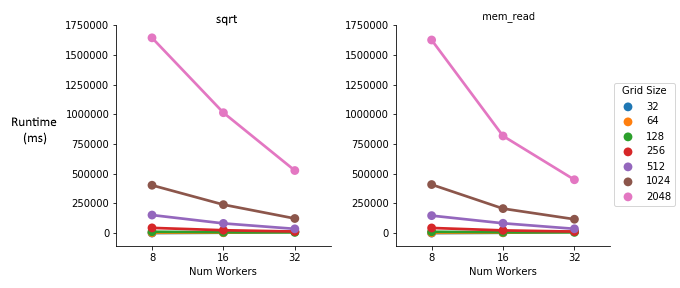
\includegraphics[width=1\textwidth]{graphics/interesting_instances/focustest2_1.png}}
    \centerline{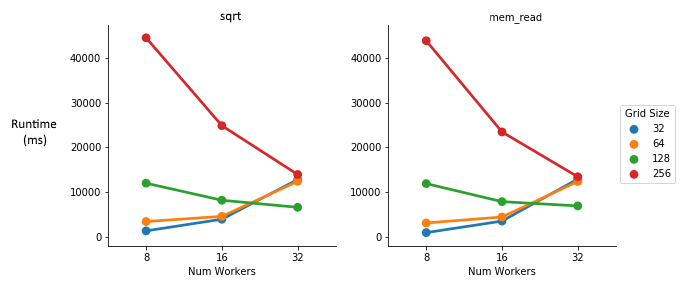
\includegraphics[width=1\textwidth]{graphics/interesting_instances/focustest2_2.png}}
    \caption{These graphs show the runtimes, in milliseconds, of various computation kernels with various grid sizes, against the number of threads used. Run on XXXII, each point is the mean of 10 repeats, with insignificant variance. We have fewer repeats with these graphs, as these graphs were part of a range whose only purpose was to let us get a feel for the performance characteristics of different kernels, such that we can select appropriate kernels for subsequent experiments.}
    \label{fig:focustest2}
\end{figure}



\begin{figure}[H]
    \centerline{
    \begin{tabular}{||c c||} 
            \hline
            \textbf{num\_runs:} & 11 \\
            \hline
            \textbf{num\_stages:} & 1 \\
            \hline
            \textbf{grid\_size:} & 32 \\
            \hline
            \textbf{num\_iterations\_0:} & 5000 \\
            \hline
            \textbf{set\_pin\_bool\_0:} & 0 \\
            \hline
            \textbf{pinnings\_0:} & - \\
            \hline
            \textbf{kernel\_repeats\_0:} & 500 \\
            \hline
            \textbf{kernel\_durations\_0:} & - \\
            \hline
            \textbf{kernels:} & sqrt \\
            \hline
            \textbf{num\_workers\_0:} & 8 \\ [1ex] 
            \hline
        \end{tabular}
    }
    \caption{The base config settings for the experiments used to select interesting grid sizes, the results of which are given in figure \ref{fig:focustest2}. Certain settings will change for different tests.}
    \label{fig:focustest2_config}
\end{figure}



As we reduce the gridsize, for both types of kernel we see a turning point around grid size 128, where increasing the thread count results in a moderate gain in performance, but with the next grid size down we lose a significant amount of performance. These are good results, as they give clear examples of cases where adding threads becomes detrimental to performance. 

However, we would also like to see if a similar effect could be had by changing the amount of computation done at each point in the grid, rather than the number of points in the grid. Both increase the total amount of work to be done, so we should see similar results. Also, this would allow more fine grained tuning of our instances.



\subsection{Selecting Interesting Kernel Complexities}
\label{section:results:selecting_interesting_kernel_complexities}

To make our kernels more complex, we simply repeat their computational core a given number of times. This gives us a linear control on the amount of work that is done at each point in the grid. Each kernel was tested with multiple grid sizes and different numbers of repeats. Varying the repeats should make our understanding of the differences between instances more fine grained, and thus, allow us to identify the point at which, as the grid size/number of repeats shrinks, increasing the number of threads would be sub-optimal. An example of the results for the sqrt (CPU stressing) kernel on XXXII is presented in figure \ref{fig:focustest3}.



\begin{figure}[H]
    \vspace*{-1.5in}
    \centerline{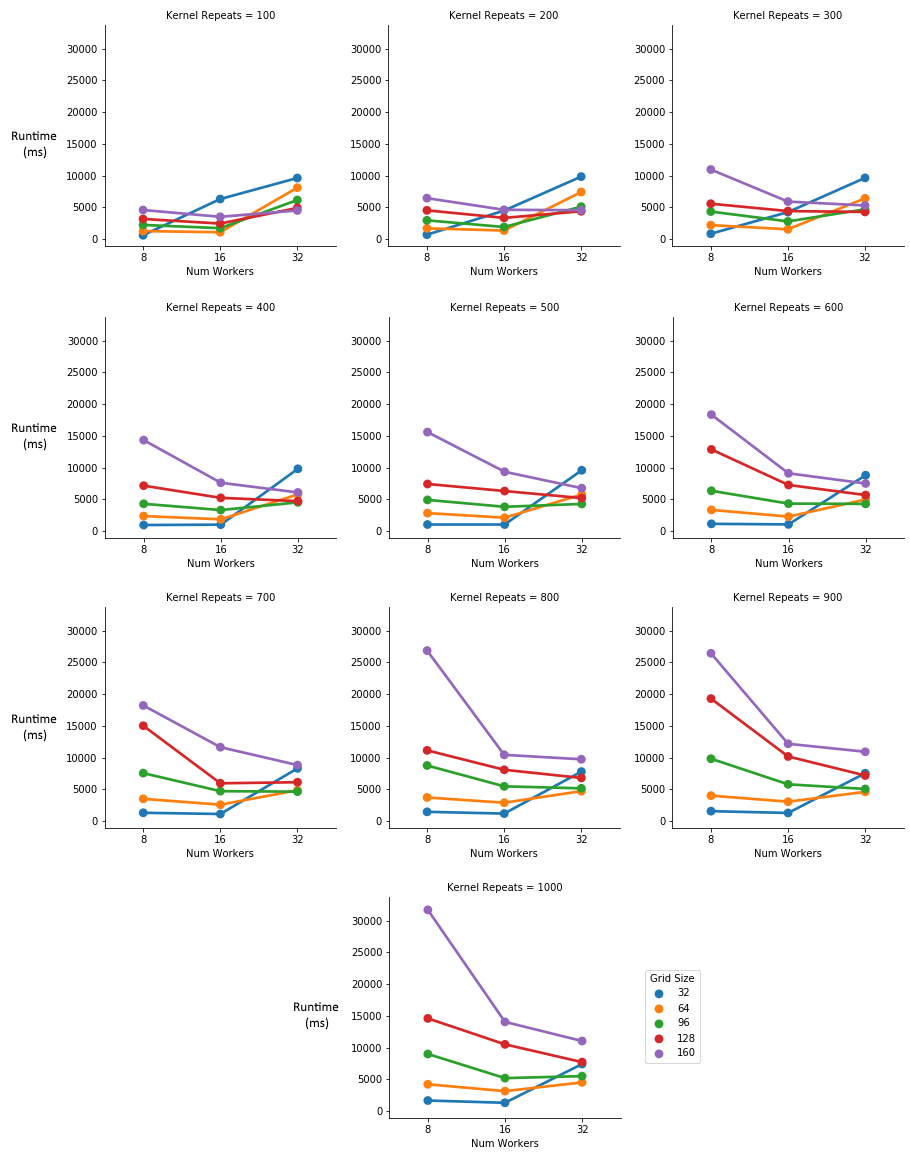
\includegraphics[width=1.3\textwidth]{graphics/interesting_instances/focustest3_2.png}}
    \caption{These graphs show the runtimes, in milliseconds, of the sqrt computation kernel with various grid sizes and various numbers of kernel repeats, against the number of threads used. Run on XXXII, each point is the mean of 10 repeats, with insignificant variance. We have fewer repeats with these graphs, as these graphs were part of a range whose only purpose was to let us get a feel for the performance characteristics of different kernels, such that we can select appropriate kernels for subsequent experiments.}
    \label{fig:focustest3}
\end{figure}



\begin{figure}[H]
    \centerline{
    \begin{tabular}{||c c||} 
            \hline
            \textbf{num\_runs:} & 11 \\
            \hline
            \textbf{num\_stages:} & 1 \\
            \hline
            \textbf{grid\_size:} & 32 \\
            \hline
            \textbf{num\_iterations\_0:} & 5000 \\
            \hline
            \textbf{set\_pin\_bool\_0:} & 0 \\
            \hline
            \textbf{pinnings\_0:} & - \\
            \hline
            \textbf{kernel\_repeats\_0:} & 100 \\
            \hline
            \textbf{kernel\_durations\_0:} & - \\
            \hline
            \textbf{kernels:} & sqrt \\
            \hline
            \textbf{num\_workers\_0:} & 8 \\ [1ex] 
            \hline
        \end{tabular}
    }
    \caption{The base config settings for the experiments used to select interesting kernel complexities, the results of which are given in figure \ref{fig:focustest3}. Certain settings will change for different tests.}
    \label{fig:focustest3_config}
\end{figure}



From figure \ref{fig:focustest3}, looking at the case with 100 kernel repeats, we can see that the graph is ``twisted.'' That is, whilst in all cases increasing threads beyond 16 degrades performance, the smaller grid sizes perform much worse with more threads, and the larger grid sizes are not affected as much. And again, as expected, we see that as the kernel complexity is increased (more kernel repeats) the graphs are slowly untwisted, since we are gradually increasing the total amount of work to be done, which lessens the ratio of overhead to useful work.

From these tests we have selected our interesting instances, ready for the next stage of experiments. These instances are:

\begin{itemize}
    \item[\textbf{CPU Small}] Uses the sqrt kernel (simply named CPU in our config) to stress the CPU. Small grid size and few kernel repeats, meaning we should encounter a point where adding threads degrades performance. Parameters are as follows:
    
    \begin{itemize}
        \item[\textit{\textbf{num\_runs:}}] 101
        
        \item[\textit{\textbf{num\_stages:}}] 1
        
        \item[\textit{\textbf{grid\_size:}}] 32
        
        \item[\textit{\textbf{kernels:}}] CPU
        
        \item[\textit{\textbf{num\_iterations\_n:}}] 1000
        
        \item[\textit{\textbf{set\_pin\_bool\_n:}}] 2
        
        \item[\textit{\textbf{kernel\_repeats\_n:}}] 75
        
        \item[\textit{\textbf{num\_workers\_n:}}] Varies
        
        \item[\textit{\textbf{pinnings\_n:}}] Varies
    \end{itemize}
    
    \item[\textbf{CPU Large}] Uses the sqrt kernel (simply named CPU in our config) to stress the CPU. Large grid size and many kernel repeats, meaning adding threads should always benefit performance. Parameters are as follows:
    
    \begin{itemize}
        \item[\textit{\textbf{num\_runs:}}] 101
        
        \item[\textit{\textbf{num\_stages:}}] 1
        
        \item[\textit{\textbf{grid\_size:}}] 256
        
        \item[\textit{\textbf{kernels:}}] CPU
        
        \item[\textit{\textbf{num\_iterations\_n:}}] 1
        
        \item[\textit{\textbf{set\_pin\_bool\_n:}}] 2
        
        \item[\textit{\textbf{kernel\_repeats\_n:}}] 1000
        
        \item[\textit{\textbf{num\_workers\_n:}}] Varies
        
        \item[\textit{\textbf{pinnings\_n:}}] Varies
    \end{itemize}
    
    \item[\textbf{VM Small}] Uses the mem\_read kernel (simply named VM in our config) to stress the virtual memory (by allocating memory and touching certain bytes). Small grid size and few kernel repeats, meaning we should encounter a point where adding threads degrades performance. Parameters are as follows:
    
    \begin{itemize}
        \item[\textit{\textbf{num\_runs:}}] 101
        
        \item[\textit{\textbf{num\_stages:}}] 1
        
        \item[\textit{\textbf{grid\_size:}}] 32
        
        \item[\textit{\textbf{kernels:}}] VM
        
        \item[\textit{\textbf{num\_iterations\_n:}}] 1000
        
        \item[\textit{\textbf{set\_pin\_bool\_n:}}] 2
        
        \item[\textit{\textbf{kernel\_repeats\_n:}}] 10
        
        \item[\textit{\textbf{num\_workers\_n:}}] Varies
        
        \item[\textit{\textbf{pinnings\_n:}}] Varies
    \end{itemize}
    
    \item[\textbf{VM Large}] Uses the mem\_read kernel (simply named VM in our config) to stress the virtual memory (by allocating memory and touching certain bytes). Large grid size and many kernel repeats, meaning adding threads should always benefit performance. Parameters are as follows:
    
    \begin{itemize}
        \item[\textit{\textbf{num\_runs:}}] 101
        
        \item[\textit{\textbf{num\_stages:}}] 1
        
        \item[\textit{\textbf{grid\_size:}}] 256
        
        \item[\textit{\textbf{kernels:}}] VM
        
        \item[\textit{\textbf{num\_iterations\_n:}}] 1
        
        \item[\textit{\textbf{set\_pin\_bool\_n:}}] 2
        
        \item[\textit{\textbf{kernel\_repeats\_n:}}] 1000
        
        \item[\textit{\textbf{num\_workers\_n:}}] Varies
        
        \item[\textit{\textbf{pinnings\_n:}}] Varies
    \end{itemize}
\end{itemize}



\section{Finding Optimal Thread Counts}
\label{section:results:finding_optimal_thread_counts}

With these experiments, the aim is to characterise the performance of each selected instance in fine detail, to give us a baseline for comparison. To this effect, we evaluate the runtime across a longer, more refined range of core counts and thread counts than in the previous section. Note - typically, programs are profiled individually, to find the optimal parameters. This experiment is akin to someone profiling a program to find the best possible performance.

As discussed in section \ref{section:design:optimal_threads}, for these experiments, we are interested in a comparison across machines. Each experiment was performed on two machines (spa and XXXII,) adjusting the maximum core/thread counts where applicable. We have one machine with 2x6 Core CPUs, with hyper-threading, for a total of 24 threads (spa,) and another with 4x8 Core CPUs, with hyper-threading, for a total of 64 threads (XXXII). The exact details of these machines can be found in section \ref{section:experimental_methodology:machine_details}. The config files used for these experiments are those from section \ref{section:results:selecting_interesting_kernel_complexities}.



\subsection{Finding the Optimal Thread Counts for the CPU Small Workload}
\label{section:results:finding_the_optimal_thread_couonts_for_the_cpu_small_workload}

Looking at the case where we have two cores in figure \ref{fig:opt_spa_cpu_small}, we can see that going above two threads only degrades performance. This is expected, since we are not adding any additional compute power, but we are adding more overhead with more threads. This continues up until we reach 6 cores. This seems to be the ``sweet spot'', where we have just the right amount of threads, and any more or any less degrades performance. This is a good result, as this is the performance characteristic we desired for the small workloads, as discussed in section \ref{section:design:interesting_instances}.

Another observation is that wherever adding threads degrades performance, we see that it degrades at the same rate. This applies in both the non-hyperthreaded graph and the hyperthreaded graph. This is consistent with what we would expect, as adding a set number of threads should add a set amount of overhead in managing those threads, and inefficiency related to contention between threads.

Interestingly, once we get into the hyperthreads, and particularly with many hyperthreads, we see a larger ``sweet spot'', that is, in the case with 24 virtual CPU cores, assigning anywhere from 8-16 threads results in decent performance. This may be due to more spatial locality, and less context switching cost due to the hyperthreads being entirely virtual, and occupying the same die location as the corresponding physical CPU core.

In profiling a program from these results, one might conclude that using around 24 cores with 12 threads would be optimal. Later, we show that this is a potential pitfall if this program is to be run in conjunction with others, where contention over resources proves to be an issue.



From figure \ref{fig:opt_xxxii_cpu_small}, we can see that for the CPU small workload, similar to the case on spa, we gain performance up to a point, and then it starts degrading as we lose threads. Interestingly, again, we have a ``sweet spot'' at around 6 threads. However, this occurs when we provide access to a large amount of cores, (26+,) and not when we restrict access to fewer virtual CPU cores (8-24.)

We can also see that once we start including hyperthreads, the performance characteristics of this workload are very regular, and perform best with 8 threads.

On the whole, these are good results, as they are in line with what we would expect.



\begin{figure}[H]
    \vspace*{-2.5cm}
    \centerline{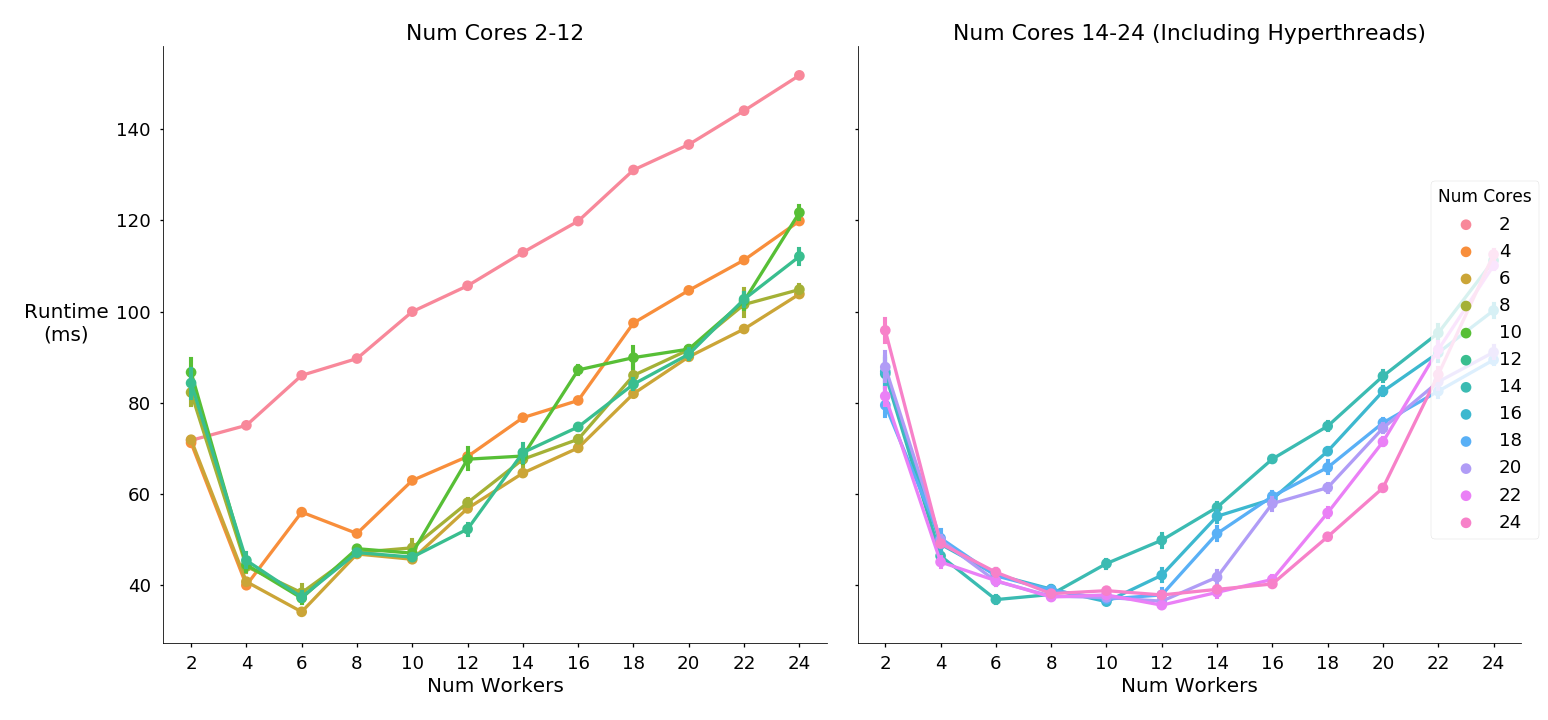
\includegraphics[width=1.5\textwidth]{graphics/optimal_threads/spa/optimal_threads_cpu_small.png}}
    \caption{Runtimes in milliseconds of the CPU small workload on spa, for varying numbers of workers (threads) and cores (virtual CPU cores.) Points are the mean of 100 values, error bars show 95\% confidence intervals. Results have been split across two graphs for clarity.}
    \label{fig:opt_spa_cpu_small}
    
    \centerline{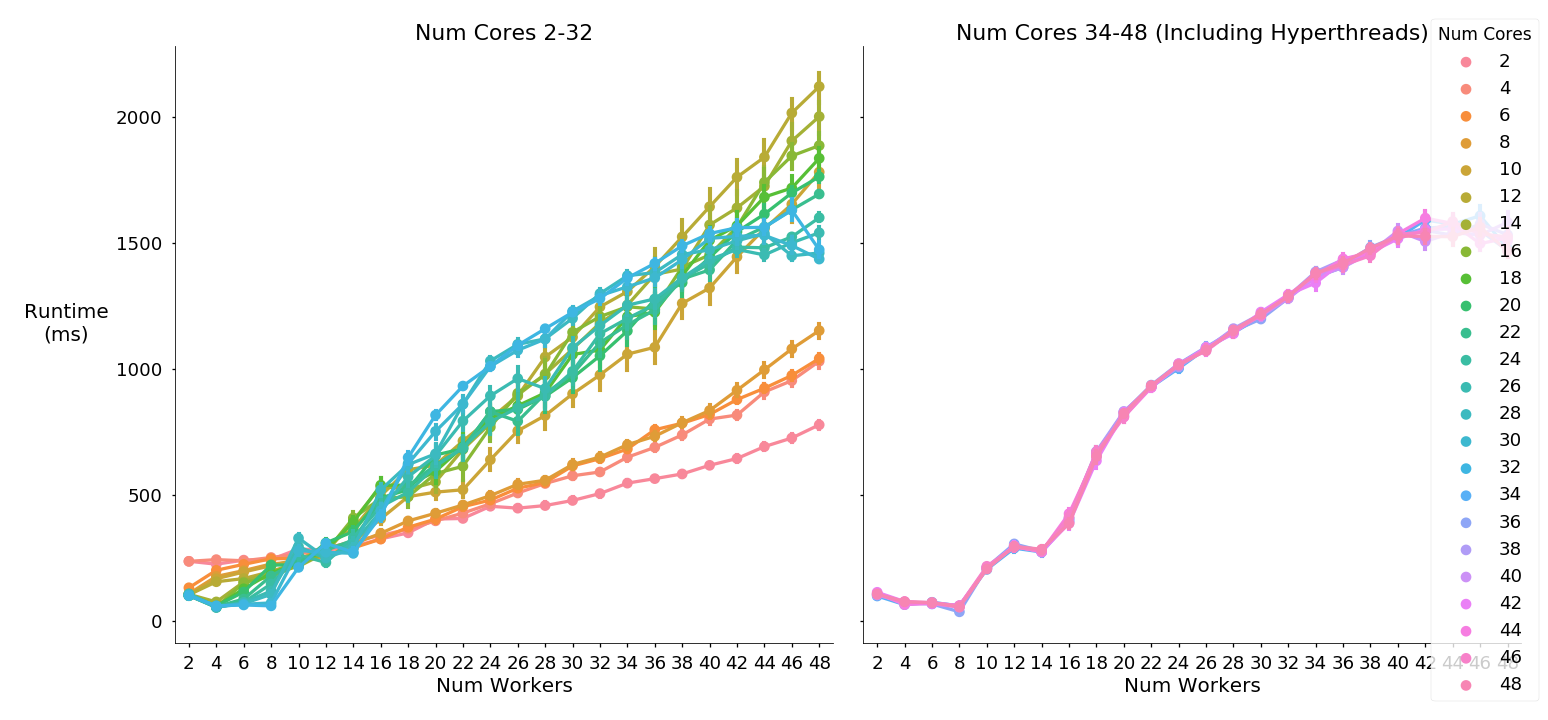
\includegraphics[width=1.5\textwidth]{graphics/optimal_threads/XXXII/optimal_threads_cpu_small.png}}
    \caption{Runtimes in milliseconds of the CPU small workload on XXXII, for varying numbers of workers (threads) and cores (virtual CPU cores.) Points are the mean of 100 values, error bars show 95\% confidence intervals. Results have been split across two graphs for clarity.}
    \label{fig:opt_xxxii_cpu_small}
\end{figure}



\subsection{Finding the Optimal Thread Counts for the CPU Large Workload}
\label{section:results:finding_the_optimal_thread_couonts_for_the_cpu_large_workload}

In contrast to the previous case, from the graphs in figure \ref{fig:opt_spa_cpu_large}, we can see that there is little to no penalty to assigning too many threads, regardless of how many CPU cores we have access to. This is because we have more work to do per iteration, meaning less contention between threads. This is described in more detail in section \ref{section:design:performance_characteristics_investigation}. Again, this is a good result, as this is a desired characteristic of the large workloads, as discussed in section \ref{section:design:interesting_instances}.

Another take away from these results is that hyperthreading does not hinder our performance, and may give some slight gain. Looking at the case with 24 virtual CPU cores, there is a significant jump in performance from the case with 22 virtual CPU cores. We cannot say why this is, as answering this question would require further investigation, and we felt our time was better spent elsewhere. If we discard this case, we do not see any benefit from utilising hyperthreading.



The results presented in figure \ref{fig:opt_xxxii_cpu_large} for XXXII resemble the results given in figure \ref{fig:opt_spa_cpu_large} for spa. In general, we see that for this workload, we do not reach the point where adding more threads would degrade performance.

However, in this case, adding more threads than cores can sometimes be beneficial, e.g. with 4 cores, using 16 threads performs substantially better than 4 threads.

Another takeaway from these graphs is that utilising hyperthreads gives us approximately the same performance as the case without. This is similar to the results from spa, if we discard the case with 24 cores.



\begin{figure}[H]
    \vspace*{-2.5cm}
    \centerline{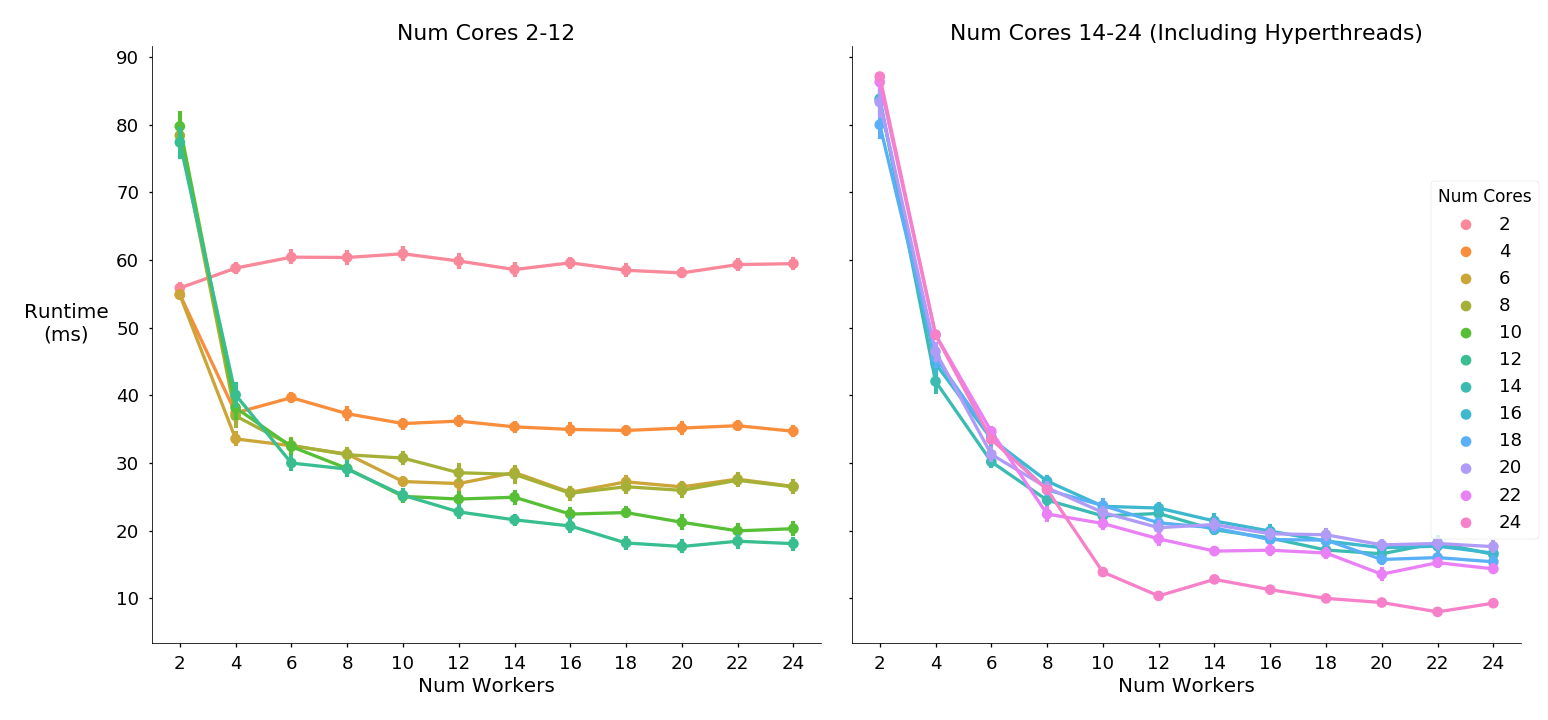
\includegraphics[width=1.5\textwidth]{graphics/optimal_threads/spa/optimal_threads_cpu_large.png}}
    \caption{Runtimes in milliseconds of the CPU large workload on spa, for varying numbers of workers (threads) and cores (virtual CPU cores.) Points are the mean of 100 values, error bars show 95\% confidence intervals. Results have been split across two graphs for clarity.}
    \label{fig:opt_spa_cpu_large}
    
    \centerline{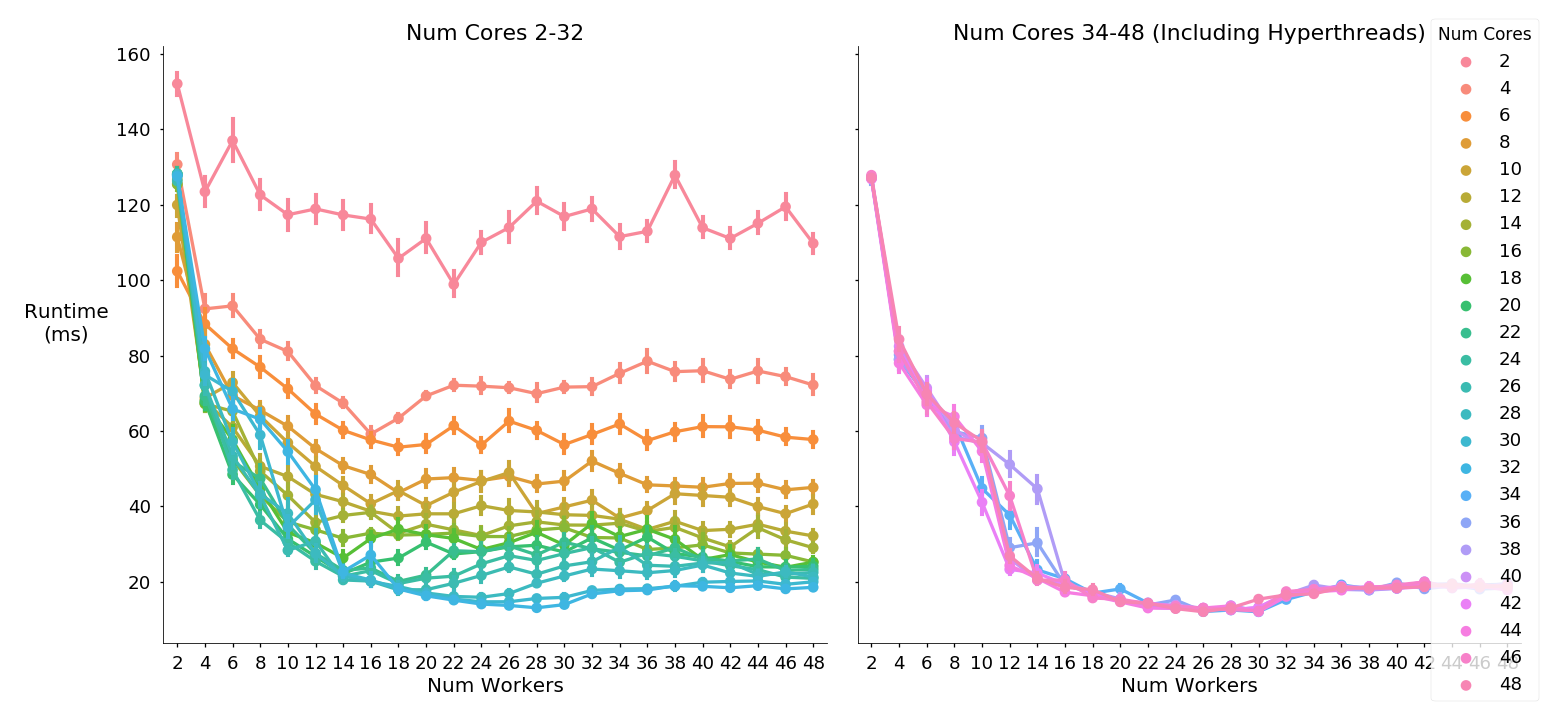
\includegraphics[width=1.5\textwidth]{graphics/optimal_threads/XXXII/optimal_threads_cpu_large.png}}
    \caption{Runtimes in milliseconds of the CPU large workload on XXXII, for varying numbers of workers (threads) and cores (virtual CPU cores.) Points are the mean of 100 values, error bars show 95\% confidence intervals. Results have been split across two graphs for clarity.}
    \label{fig:opt_xxxii_cpu_large}
\end{figure}



\subsection{Finding the Optimal Thread Counts for the VM Small Workload}
\label{section:results:finding_the_optimal_thread_couonts_for_the_vm_small_workload}

Comparing the graphs in figure \ref{fig:opt_spa_vm_small} to the previous cases, we can see similarities to both. Similar to the first case, we can see that, at least for the case without hyperthreads, there is a point at which adding more threads degrades performance. Indeed, again it seems to be at 6 cores/threads. Another similarity is that, again for the case without hyperthreads, adding more threads than we have cores generally degrades performance. However, the degradation is not as steady, or even in the case where we have access to 12 cores, we do not see much degradation at all.

We can see reasonable scaling of performance with the number of workers, up until we reach 6 cores/threads. Here, our performance plateaus, suggesting that the critical resource, in this case the virtual memory of the system, is saturated.

In the case where we have access to hyperthreads, interestingly we see that there is clear, tangible, benefit, in that we obtain our fastest runtimes. Perhaps hyperthreading, which allows threads in the same die location on the CPU to share data, facilitates efficient data use. In general, a strategy of assigning as many cores and threads as we can would be reasonable, as we only just start to see some performance degradation as we approach 24 threads in the case where we have access to 24 cores. However, we expect this to change when the program is run in contention with others.



The results presented in \ref{fig:opt_xxxii_vm_small} tell a similar story to those in \ref{fig:opt_spa_vm_small}, in that they seem to follow a regular pattern, that with providing access to more virtual CPU cores, we do not gain more performance, but rather a bigger ``sweet spot'', where we can allocate more threads without losing performance. Again, this large ``sweet spot'' suggests that the critical resource (the virtual memory) is saturated.

However these results do present some oddities. For example, in the case where we have access to two virtual CPU cores, the performance varies wildly with different numbers of workers, with a large amount of variance. This variance may be due to the cost of memory operations changing, as we have a large amount of threads running on just two cores, meaning that there are many context switches between threads. We see a similar pattern when we have access to four virtual CPU cores, however, once we are past four, we settle into the regular pattern, and when we start utilising hyperthreading, we neither lose nor gain performance. This is in contrast to the results from spa, as in that case, we could both lose or gain performance.



\begin{figure}[H]
    \vspace*{-2.5cm}
    \centerline{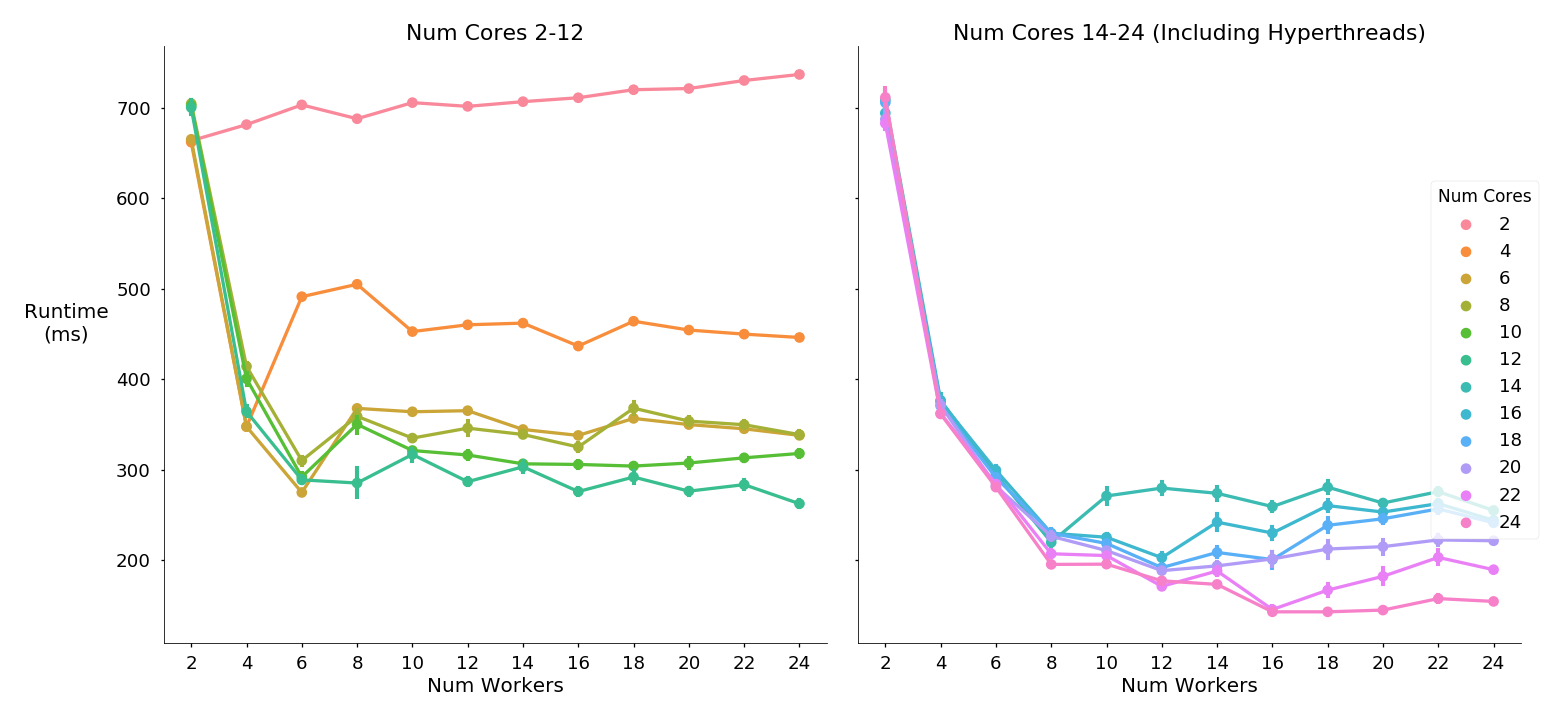
\includegraphics[width=1.5\textwidth]{graphics/optimal_threads/spa/optimal_threads_vm_small.png}}
    \caption{Runtimes in milliseconds of the VM small workload on spa, for varying numbers of workers (threads) and cores (virtual CPU cores.) Points are the mean of 100 values, error bars show 95\% confidence intervals. Results have been split across two graphs for clarity.}
    \label{fig:opt_spa_vm_small}
    
    \centerline{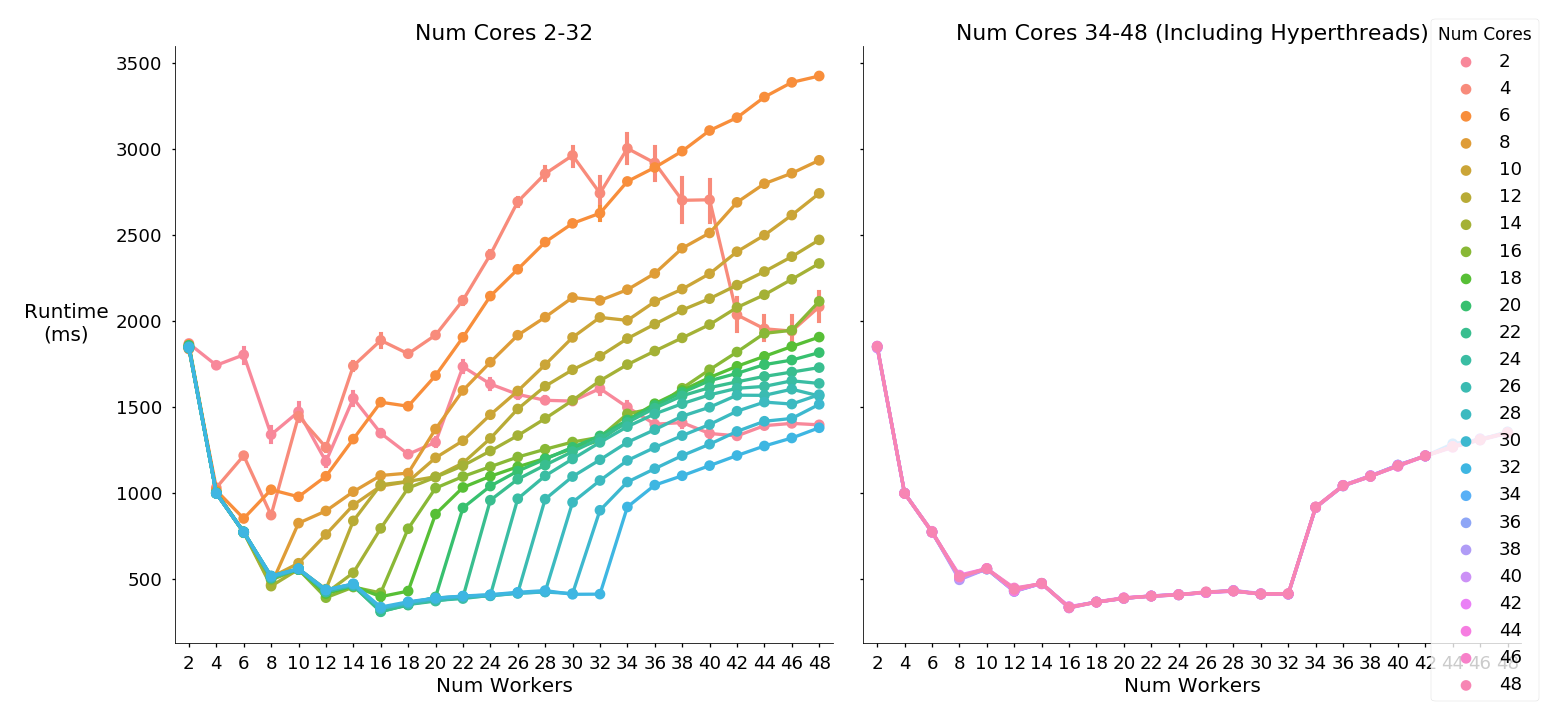
\includegraphics[width=1.5\textwidth]{graphics/optimal_threads/XXXII/optimal_threads_vm_small.png}}
    \caption{Runtimes in milliseconds of the VM small workload on XXXII, for varying numbers of workers (threads) and cores (virtual CPU cores.) Points are the mean of 100 values, error bars show 95\% confidence intervals. Results have been split across two graphs for clarity.}
    \label{fig:opt_xxxii_vm_small}
\end{figure}



\subsection{Finding the Optimal Thread Counts for the VM Large Workload}
\label{section:results:finding_the_optimal_thread_couonts_for_the_vm_large_workload}

In the graphs given in figure \ref{fig:opt_spa_vm_large}, we see the most consistent performance scaling yet. With only minor variance, we see that all cases start by following the same performance curve. When we assign more threads than virtual CPU cores, we see each curve level off, indicating that assigning more threads than cores has little to no penalty. 

Again, we see reasonable scaling of performance up to a point, and then it starts to slow. Compare the runtimes for 6 threads (approximately 1500ms) and for 12 (approximately 900ms,) The performance is not quite scaling as expected, suggesting that the critical resource, in this case the virtual memory of the system, is beginning to be saturated.

Another aspect of these graphs is that hyperthreading, again, gives us a tangible benefit, as was the case with our previous VM workload. However, it is not nearly as substantial.



These results in figure \ref{fig:opt_xxxii_vm_large} closely resemble those from spa, \ref{fig:opt_spa_vm_large}. In fact, almost all of the same conclusions can be drawn from these. However, we see much clear evidence of the critical resource becoming saturated, as we do not significantly improve our performance going above 20 threads.



\begin{figure}[H]
    \vspace*{-2.5cm}
    \centerline{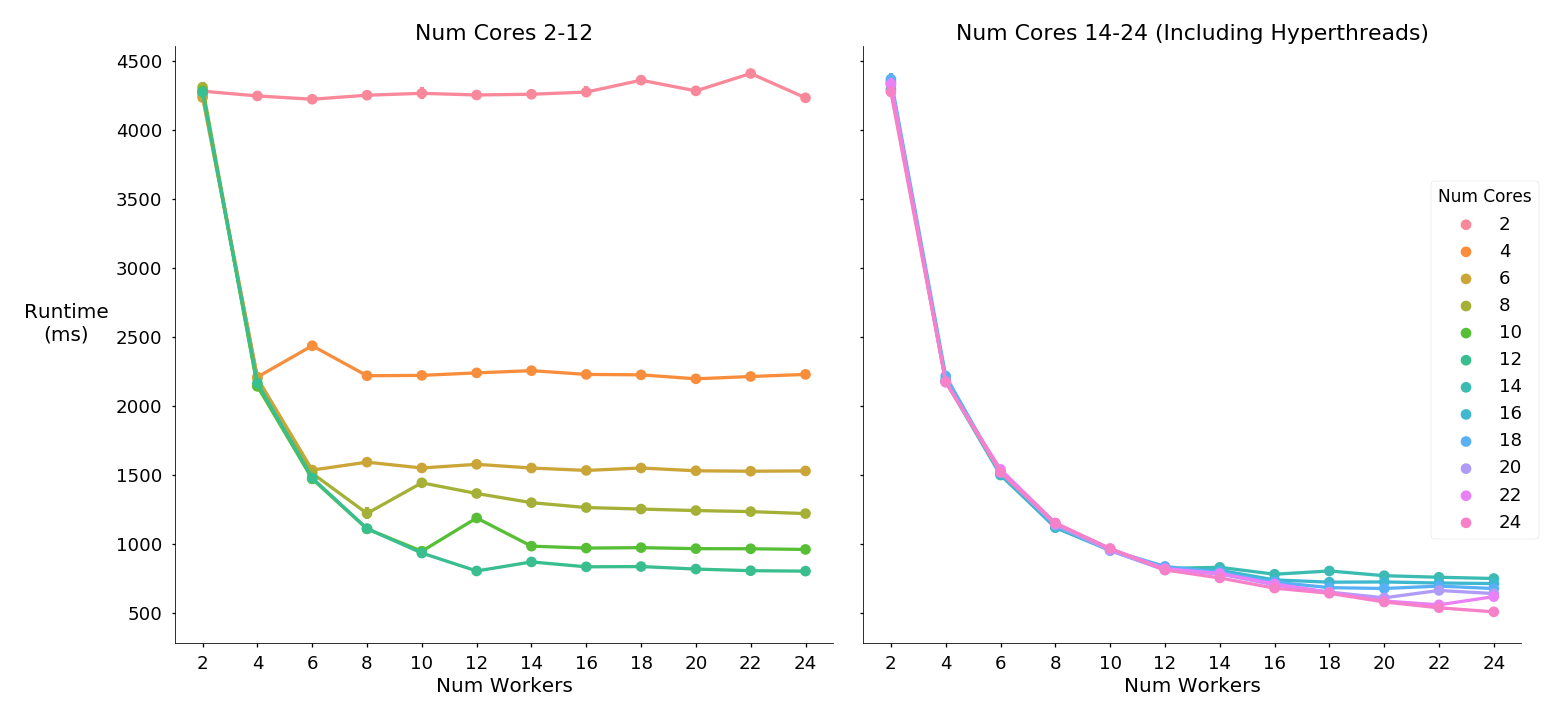
\includegraphics[width=1.5\textwidth]{graphics/optimal_threads/spa/optimal_threads_vm_large.png}}
    \caption{Runtimes in milliseconds of the VM large workload on spa, for varying numbers of workers (threads) and cores (virtual CPU cores.) Points are the mean of 100 values, error bars show 95\% confidence intervals. Results have been split across two graphs for clarity.}
    \label{fig:opt_spa_vm_large}
    
    \centerline{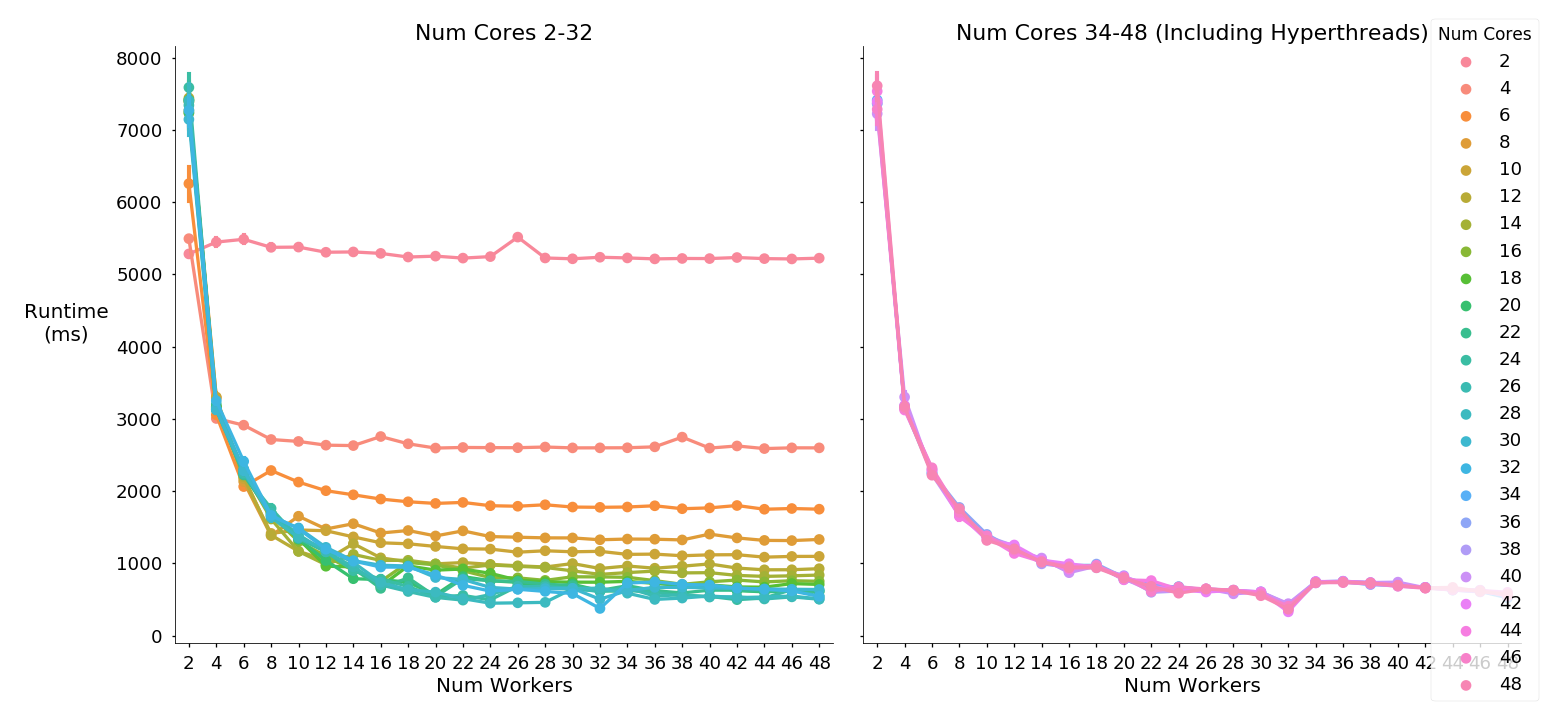
\includegraphics[width=1.5\textwidth]{graphics/optimal_threads/XXXII/optimal_threads_vm_large.png}}
    \caption{Runtimes in milliseconds of the VM large workload on XXXII, for varying numbers of workers (threads) and cores (virtual CPU cores.) Points are the mean of 100 values, error bars show 95\% confidence intervals. Results have been split across two graphs for clarity.}
    \label{fig:opt_xxxii_vm_large}
\end{figure}



\subsection{Overall Conclusion}
\label{section:results:overall_conclusion}

From these results, we can see that when a program is run in isolation, there is no disadvantage to providing the program with more cores than necessary. This may be because, whilst modern schedulers are not explicitly contention aware, they do aim to minimise unnecessary context switches, meaning that even with access to more CPU cores, we may not see increased overhead.

Both of our VM workloads have shown signs of the critical resource (the memory of the system) becoming saturated, it will be interesting to see how running these programs in contention affects their performance characteristics.

The intention of these experiments is to ascertain the performance characteristics of these programs when run in isolation, such that we can perform a direct comparison to their performance when run in contention with others. These results achieve that, we can use them as if we were profiling each program, to select the best parameters. For our contention experiments, we will see how choosing the optimal parameters for each program when they were run in isolation compares to the overall optimal parameters, when we take into account contention.



\section{Contention Experiments}
\label{section:results:contention_experiments}

In this section, we present the results of the contention experiments, as described in section \ref{section:design:contention_experiments}. These experiments are designed to assess the performance of two programs running in contention, with different assignments of threads and cores. To do this, we start both programs simultaneously, measuring overall performance in terms of throughput, by summing the runtimes of each program. This is done for each combination of values for the number of workers and the number of cores for each program.

Recall that the purpose of these experiments is to investigate if and how much we could improve performance by taking program contention into account in scheduling. To do this, we will find the performance of the case where we take each programs best settings from data corresponding to them running in isolation, (i.e. find the best number of cores / threads to use from the previous graphs,) and we want to compare this to the case which gave us the best performance when they are run simultaneously (i.e., in contention.) The difference between these two cases is how much we could improve by taking contention into account.

We intended to present results from multiple machines (spa and XXXII,) however due to time constraints, we could not complete the experiments on XXXII. This is because on spa, incrementing the number of workers and the number of cores in steps of four, we have six values to evaluate (4 - 24.) With two programs, we have four variables to alter, so this results in $6^4 = 1296$ experiments. On XXXII, we have twelve values to vary (4 - 48,) so this results in $12^4 = 20,736$. Since the experiments on spa took around a week to complete, we felt our time was better spent on other aspects of the project.

Presenting these results is complex, since we have five variables in our experiments, the number of cores for each program, the number of workers for each program, and the total runtime. To present this, for the graph of each experiment, we fix the number of cores assigned to each program to whatever gave us the best overall runtime (note - from the previous experiments, assigning more cores than threads did not do very much, meaning that the number of cores assigned is of lesser importance.) Then we produce a 3D plot of the data, varying the number of workers assigned to each program. This surface will give us some insight into the ``performance space'' of our applications. Finally, we plot two points, one showing the runtime of the individually profiled case (in purple,) and the other showing the runtime of the optimal case (in red.) 

The config files used for these experiments are combinations of those from section \ref{section:results:selecting_interesting_kernel_complexities}.



\subsection{Evaluating CPU Large and VM Large in Contention}
\label{section:results:evaluating_cpu_large_and_vm_large_in_contention}

The results presented in figure \ref{fig:con_spa_cpu_large_and_vm_large} should show little contention, as the workloads used (CPU large and VM large) stress different resources, meaning that they are not competing, so we should be able to use the data from each program running in isolation to make a good prediction of the optimal parameters. We can see that this is indeed the case, as we only see a speedup of 1.03 between the the individually profiled case (the purple dot) and the optimal configuration (the red dot.)

We can see in this graph that we have two performance curves which show that adding threads improves performance. The first, for CPU large, is very clear, and is the biggest factor in minimising the runtime. The second, for VM large, can be seen along the top edge, where the number of workers for CPU large is four. 

These results tell us that, for workloads which do not compete for the same resource, our contention aware plastic parallel programming library cannot provide a significant improvement. However, we also would not lose any performance, meaning other programs may still benefit, even if this pair will not.



\begin{figure}[H]
    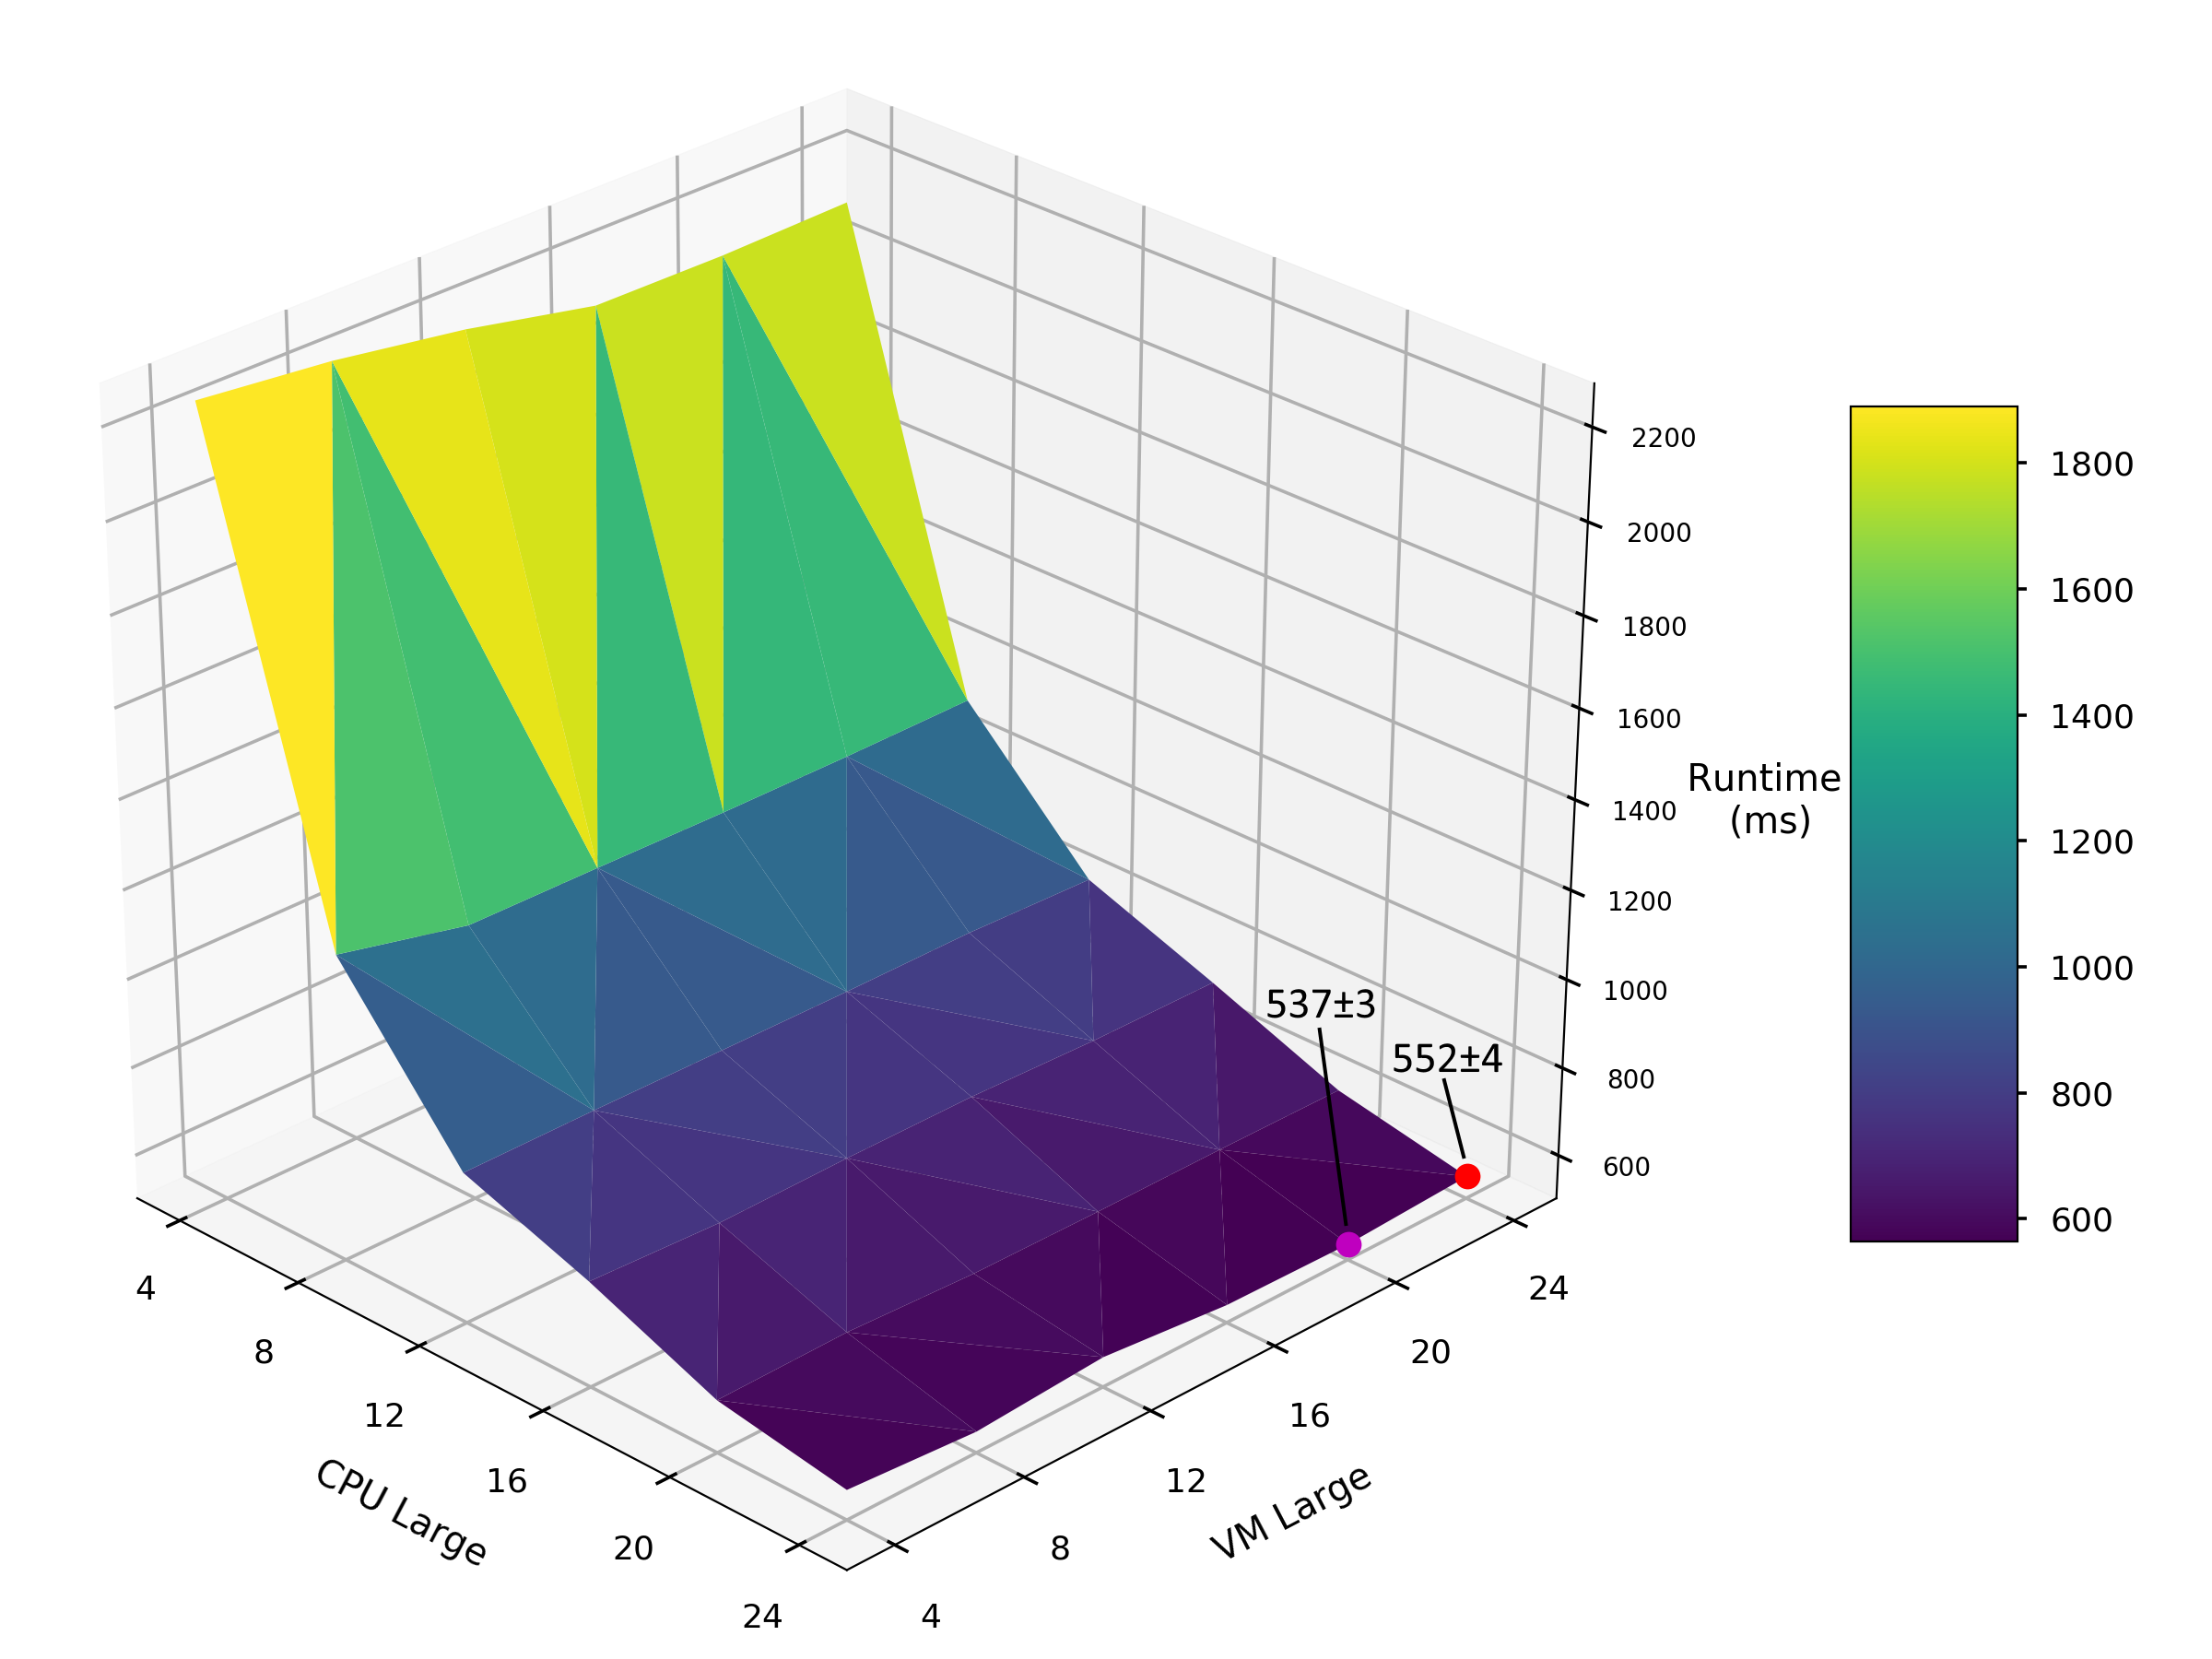
\includegraphics[width=1\textwidth]{graphics/contention/spa/otwc_cpu_large_and_vm_large.png}
    \caption{A 3D graph showing the total (summed) runtimes in milliseconds of the CPU large and VM large workloads running in contention on spa, and how they are affected by the number of workers assigned to each program. The red dot shows the result we would get if we used settings which were optimal when these programs were run in isolation. The purple dot shows the overall optimal case, which comparatively has a speedup of 1.03. This is what we could gain with a contention aware plastic parallel programming library. \\
    These results represent the case where the number of cores assigned to each program is optimal, (in this case, num cores for CPU large = 24 and num cores for VM large = 24.) Each point is the mean of 100 runs, with insignificant variance.}
    \label{fig:con_spa_cpu_large_and_vm_large}
\end{figure}



\subsection{Evaluating CPU Small and CPU Large in Contention}
\label{section:results:evaluating_cpu_small_and_cpu_large_in_contention}

The results presented in figure \ref{fig:con_spa_cpu_small_and_cpu_large} show the characteristics of the CPU small and CPU large workloads when run in contention. These workloads directly compete for resources, and as such, here we expect to see the possibility for improvement. Indeed, this is the case, with a huge speedup of 2.44, and very different parameters (independent case: CPU small num\_cores: 20, CPU small num\_workers: 12, CPU large num\_cores: 24, CPU large num\_workers: 24, optimal case: CPU small num\_cores: 24, CPU small num\_workers: 20, CPU large num\_cores: 20, CPU large num\_workers: 12.)

This large change in parameters may be surprising at first, however, from looking at the topology of the graph, the downwards slope from 24 threads for CPU large makes sense. Since CPU large can generally occupy all the cores it can get, we must reduce them in order for CPU small to get its fair share, allowing us to run both programs simultaneously and saturate the entire machine, improving our performance. Also, recall that on spa, we have 12 physical CPU cores and 24 virtual ones. So, when programs are run in isolation, we may gain a tangible benefit from utilising hyperthreading. That is, by assigning more threads than physical CPU cores. Indeed, looking at our previous results for CPU large on spa (section \ref{fig:opt_spa_cpu_large},) we may be able to gain a slight edge. However, when run in contention where CPU cores are at a premium, this is unlikely to be an optimal strategy. All this helps explain the change in threads for CPU large from the independent case (red dot) and the optimal case (purple dot.)

Looking at the topology of the graph again, we can see that there is a trough in which we can change the number of threads for CPU small, without impacting the runtime too significantly. This explains the change in threads for CPU small from the independent case (red dot) and the optimal case (purple dot.) A reason for this trough may be that the runtime of these programs running in conjunction is dominated by CPU large, and whilst there are slopes in this trough, they are simply not as significant.

These results show us that for contentious workloads, there is a large potential for improvement, and that if one workload dominates the other in the competition for resources, (in this case, CPU large dominates,) the parameters we should set for it are more critical to our overall performance, as they must enable the sharing of resources.



\begin{figure}[H]
    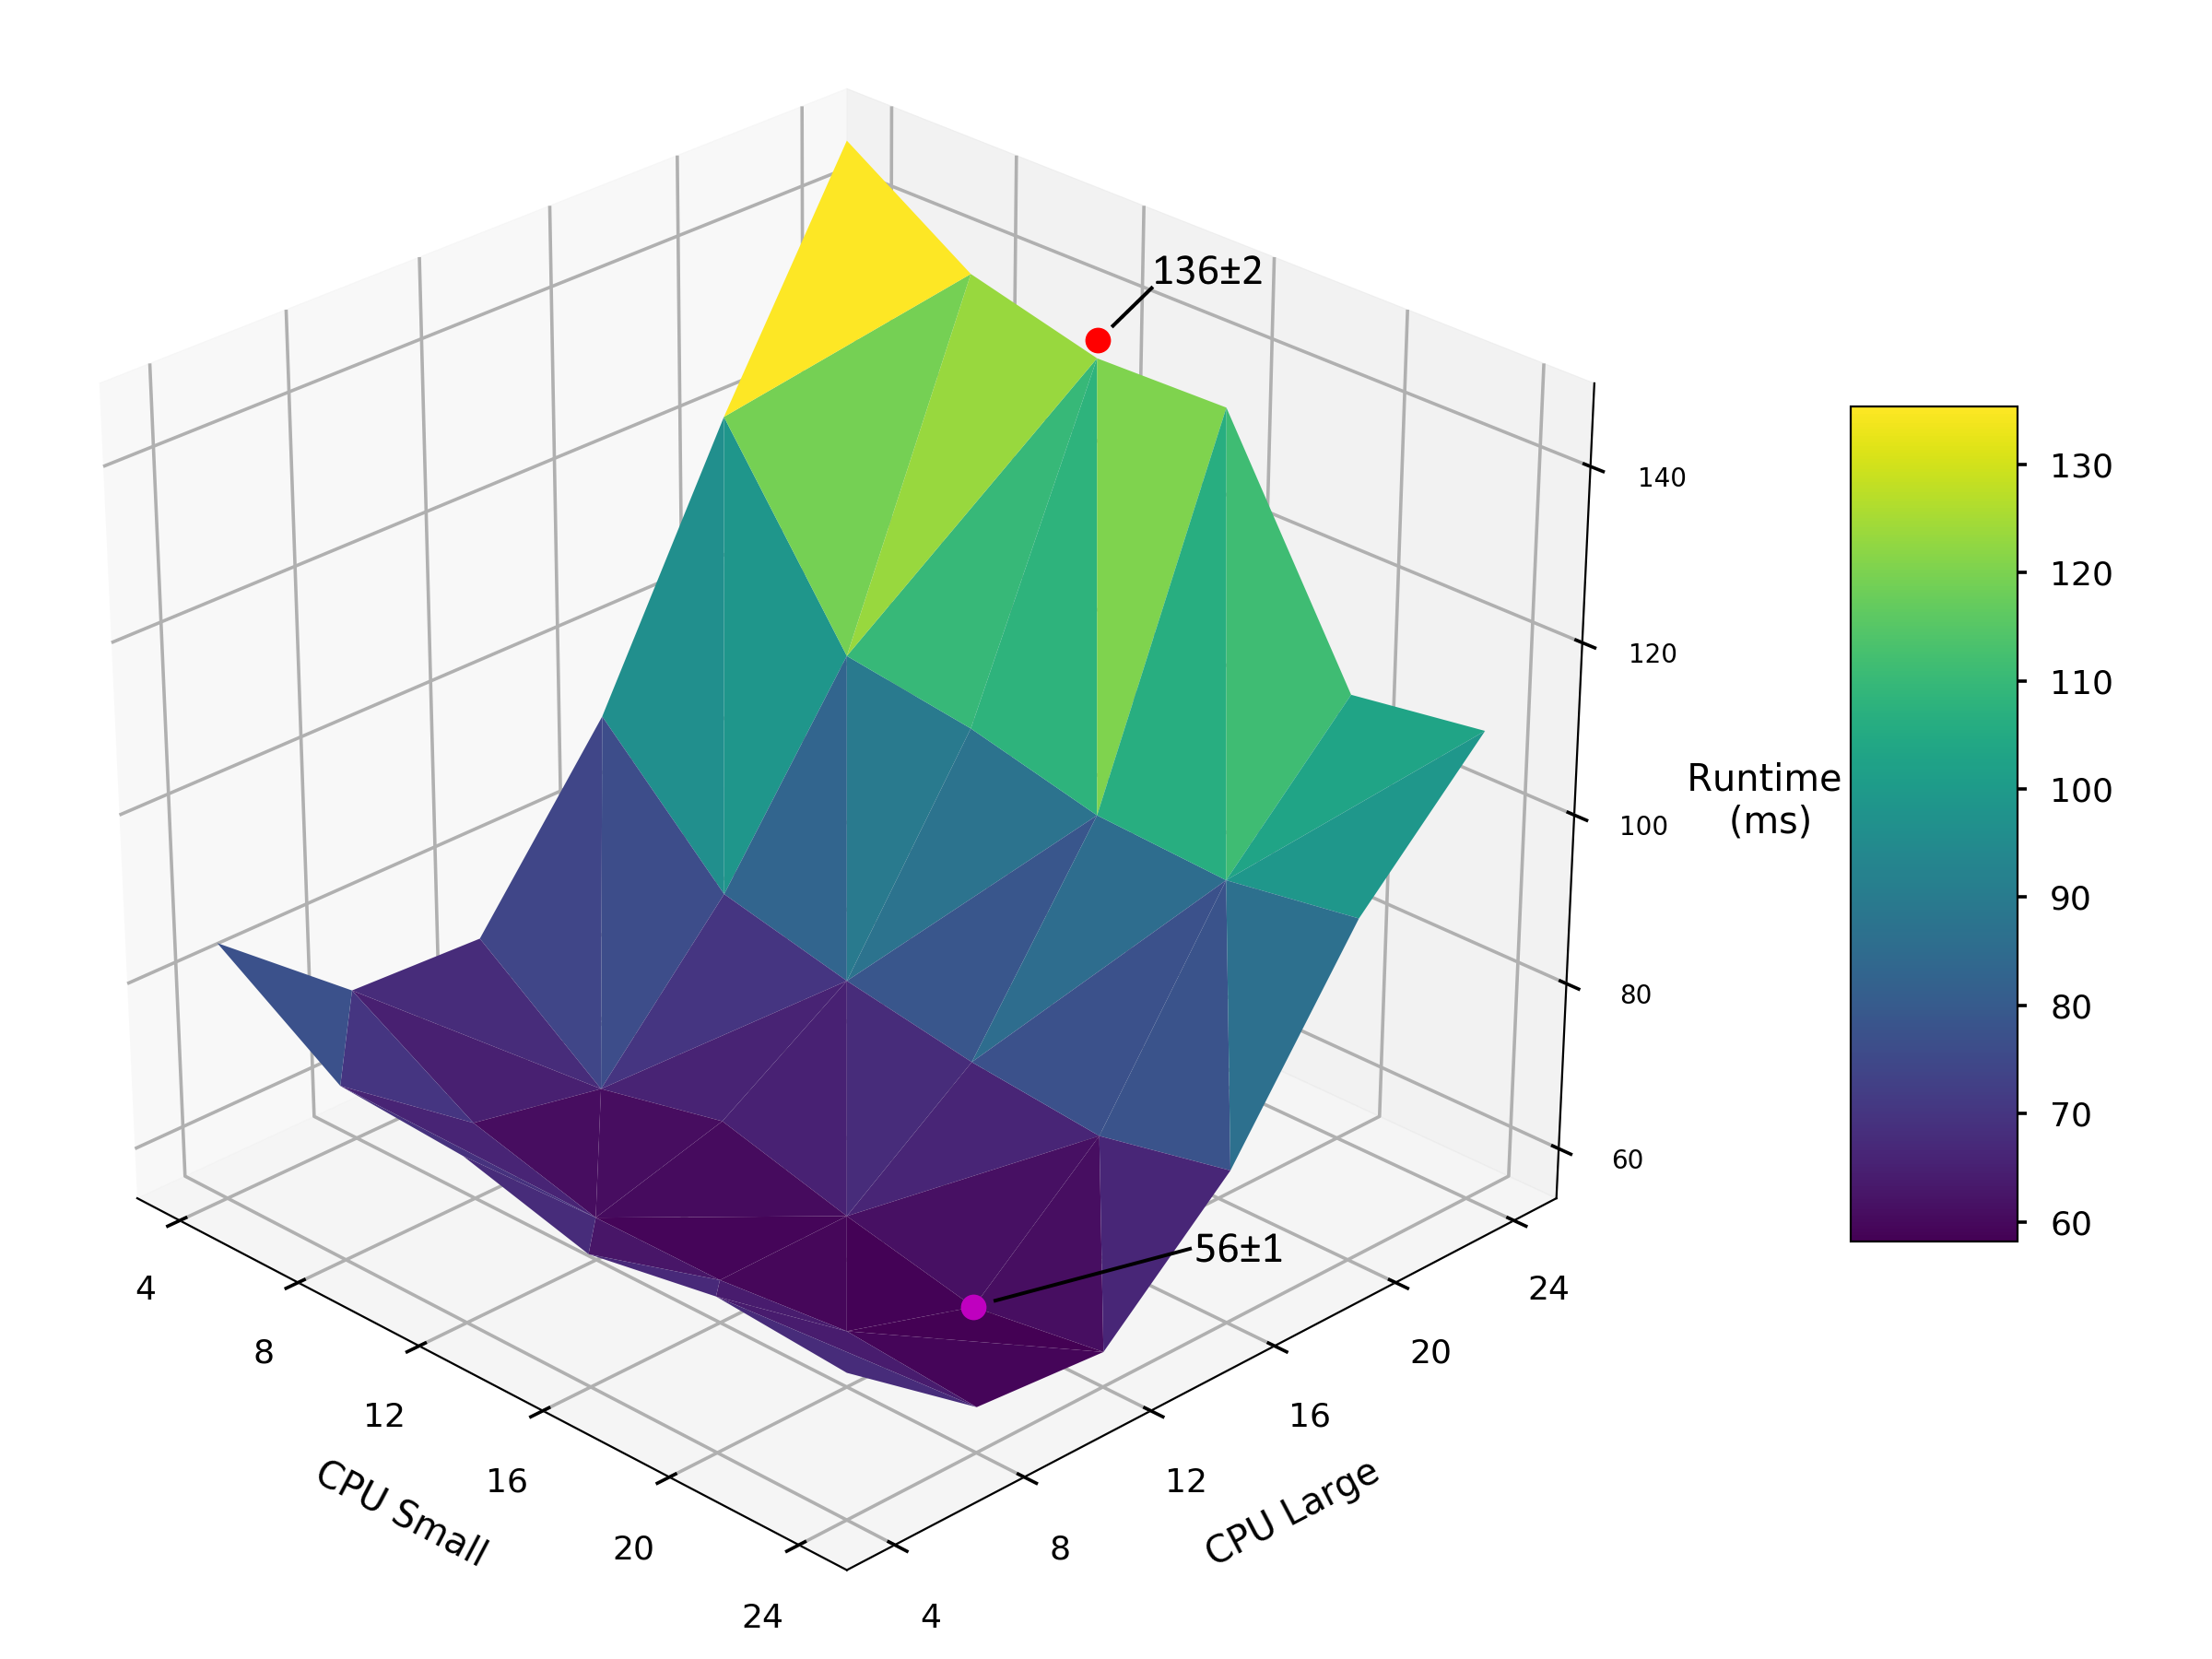
\includegraphics[width=1\textwidth]{graphics/contention/spa/otwc_cpu_small_and_cpu_large.png}
    \caption{A 3D graph showing the total (summed) runtimes in milliseconds of the CPU small and CPU large workloads running in contention on spa, and how they are affected by the number of workers assigned to each program. The red dot shows the result we would get if we used settings which were optimal when these programs were run in isolation. The purple dot shows the overall optimal case, which comparatively has a speedup of 2.44. This is what we could gain with a contention aware plastic parallel programming library. \\
    These results represent the case where the number of cores assigned to each program is optimal, (in this case, num cores for CPU small = 24 and num cores for CPU large = 20.) Each point is the mean of 100 runs, with insignificant variance.}
    \label{fig:con_spa_cpu_small_and_cpu_large}
\end{figure}



\subsection{Evaluating CPU Small and VM Small in Contention}
\label{section:results:evaluating_cpu_small_and_vm_small_in_contention}

We would expect that, since our two workloads do not directly compete for the same system resources, we would not see much improvement or difference between the individually profiled case and the optimal case. However, looking at the results in figure \ref{fig:con_spa_cpu_small_and_vm_small}, we can see that this is not the case. Indeed, we see a significant speedup of 1.60. 

It seems that the performance characteristics of our small workloads significantly change when they are run in conjunction with other programs. From the graph, we can see that the ``sweet spot'' for the CPU small workload is not around 16 workers, as opposed to 6 (from the individually profiled case.) This may be because, unlike our large workloads, the small ones are ``balanced'' at their sweet spot, and this relates to other factors, notably CPU speed. If another program is running, the small workload will get less CPU time, analogous to the CPU speed decreasing. It is plausible then that the sweet spot would shift, as the balance has changed.

These results tell us that for ``small'' workloads, (that is, workloads where adding threads is not an optimal strategy,) their performance characteristics when run in contention can change, and getting the parameters right is important. This shows promise for our contention aware plastic parallel programming library.



\begin{figure}[H]
    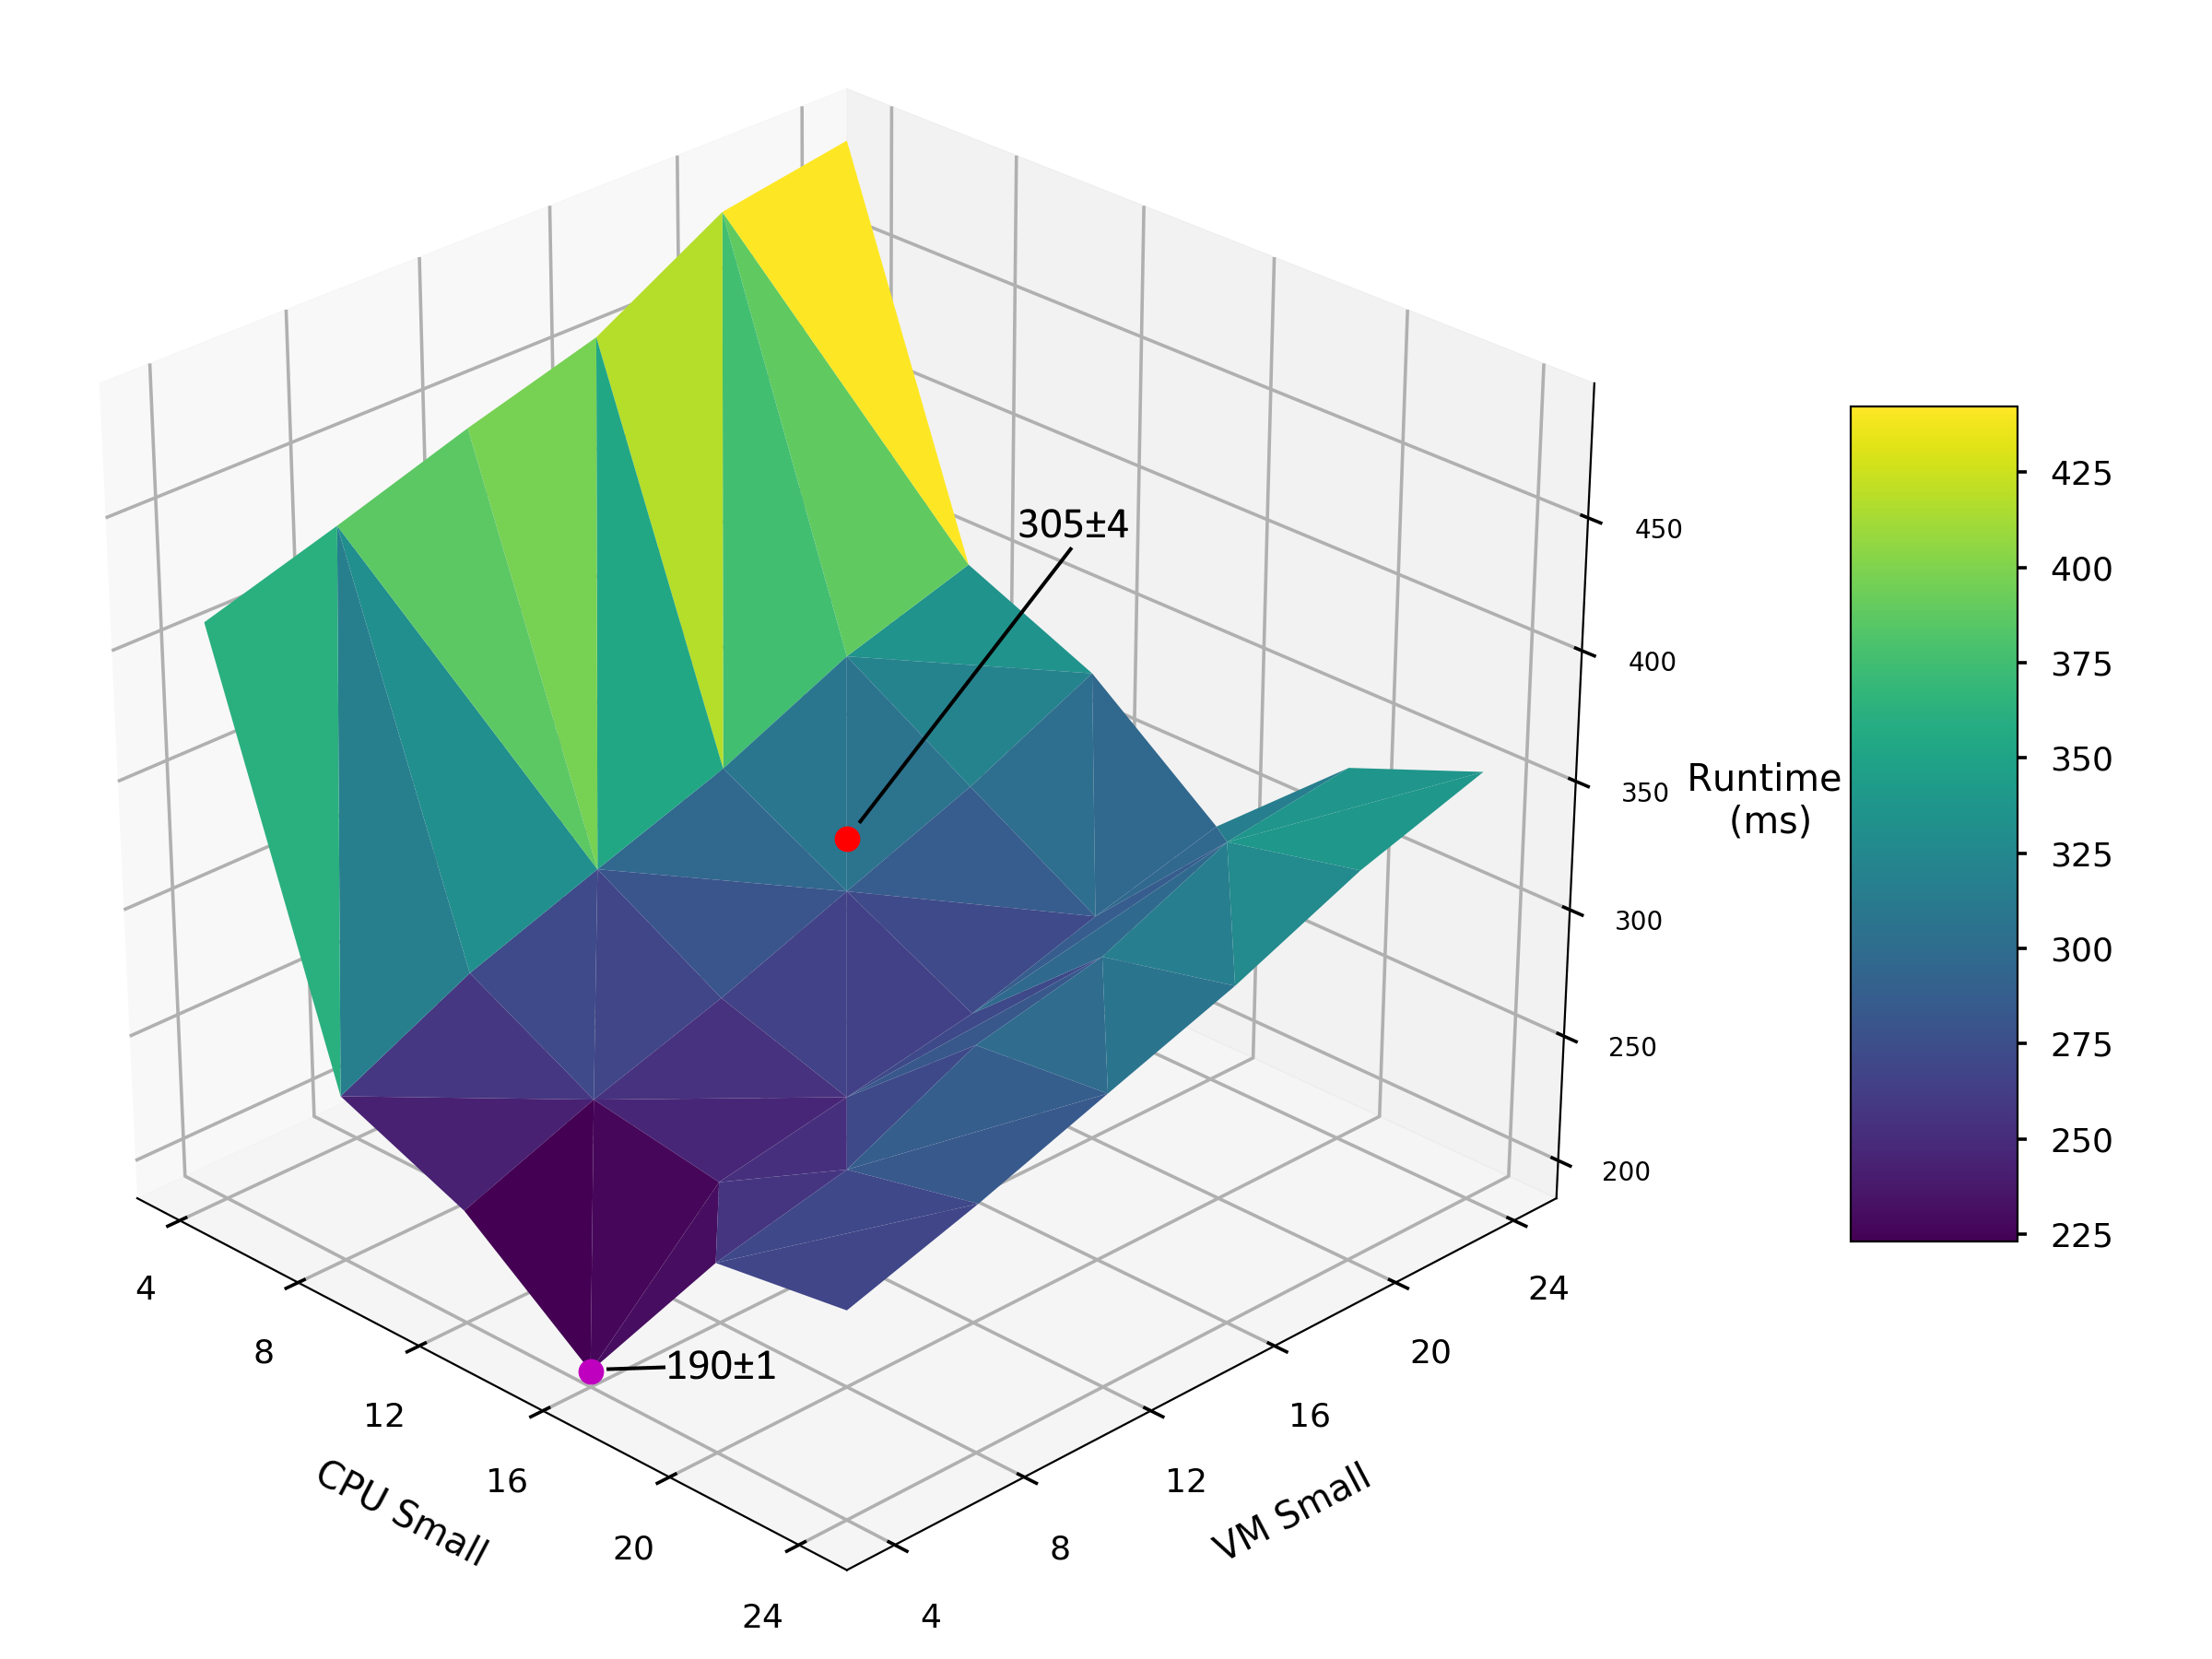
\includegraphics[width=1\textwidth]{graphics/contention/spa/otwc_cpu_small_and_vm_small.png}
    \caption{A 3D graph showing the total (summed) runtimes in milliseconds of the CPU small and VM small workloads running in contention on spa, and how they are affected by the number of workers assigned to each program. The red dot shows the result we would get if we used settings which were optimal when these programs were run in isolation. The purple dot shows the overall optimal case, which comparatively has a speedup of 1.60. This is what we could gain with a contention aware plastic parallel programming library. \\
    These results represent the case where the number of cores assigned to each program is optimal, (in this case, num cores for CPU small = 24 and num cores for VM small = 4.) Each point is the mean of 100 runs, with insignificant variance.}
    \label{fig:con_spa_cpu_small_and_vm_small}
\end{figure}



\subsection{Evaluating VM Small and CPU Large in Contention}
\label{section:results:evaluating_vm_small_and_cpu_large_in_contention}

The VM small and CPU large workloads, again, do not directly compete for system resources. Indeed, from figure \ref{fig:con_spa_vm_small_and_cpu_large}, we can see that the VM small workload has little effect on the total runtime, and that it is mostly affected by the CPU large workload. We do, however, see a substantial speedup of 1.22. This is not as drastic an improvement as seen in our previous cases, and we can also see that the values for the parameters of each program are reasonably close, but this small change still marks a valuable improvement.

These results again show us that the performance characteristics of our small workloads significantly change when run in conjunction with other programs, and that there is potential for a compelling gain in performance.



\begin{figure}[H]
    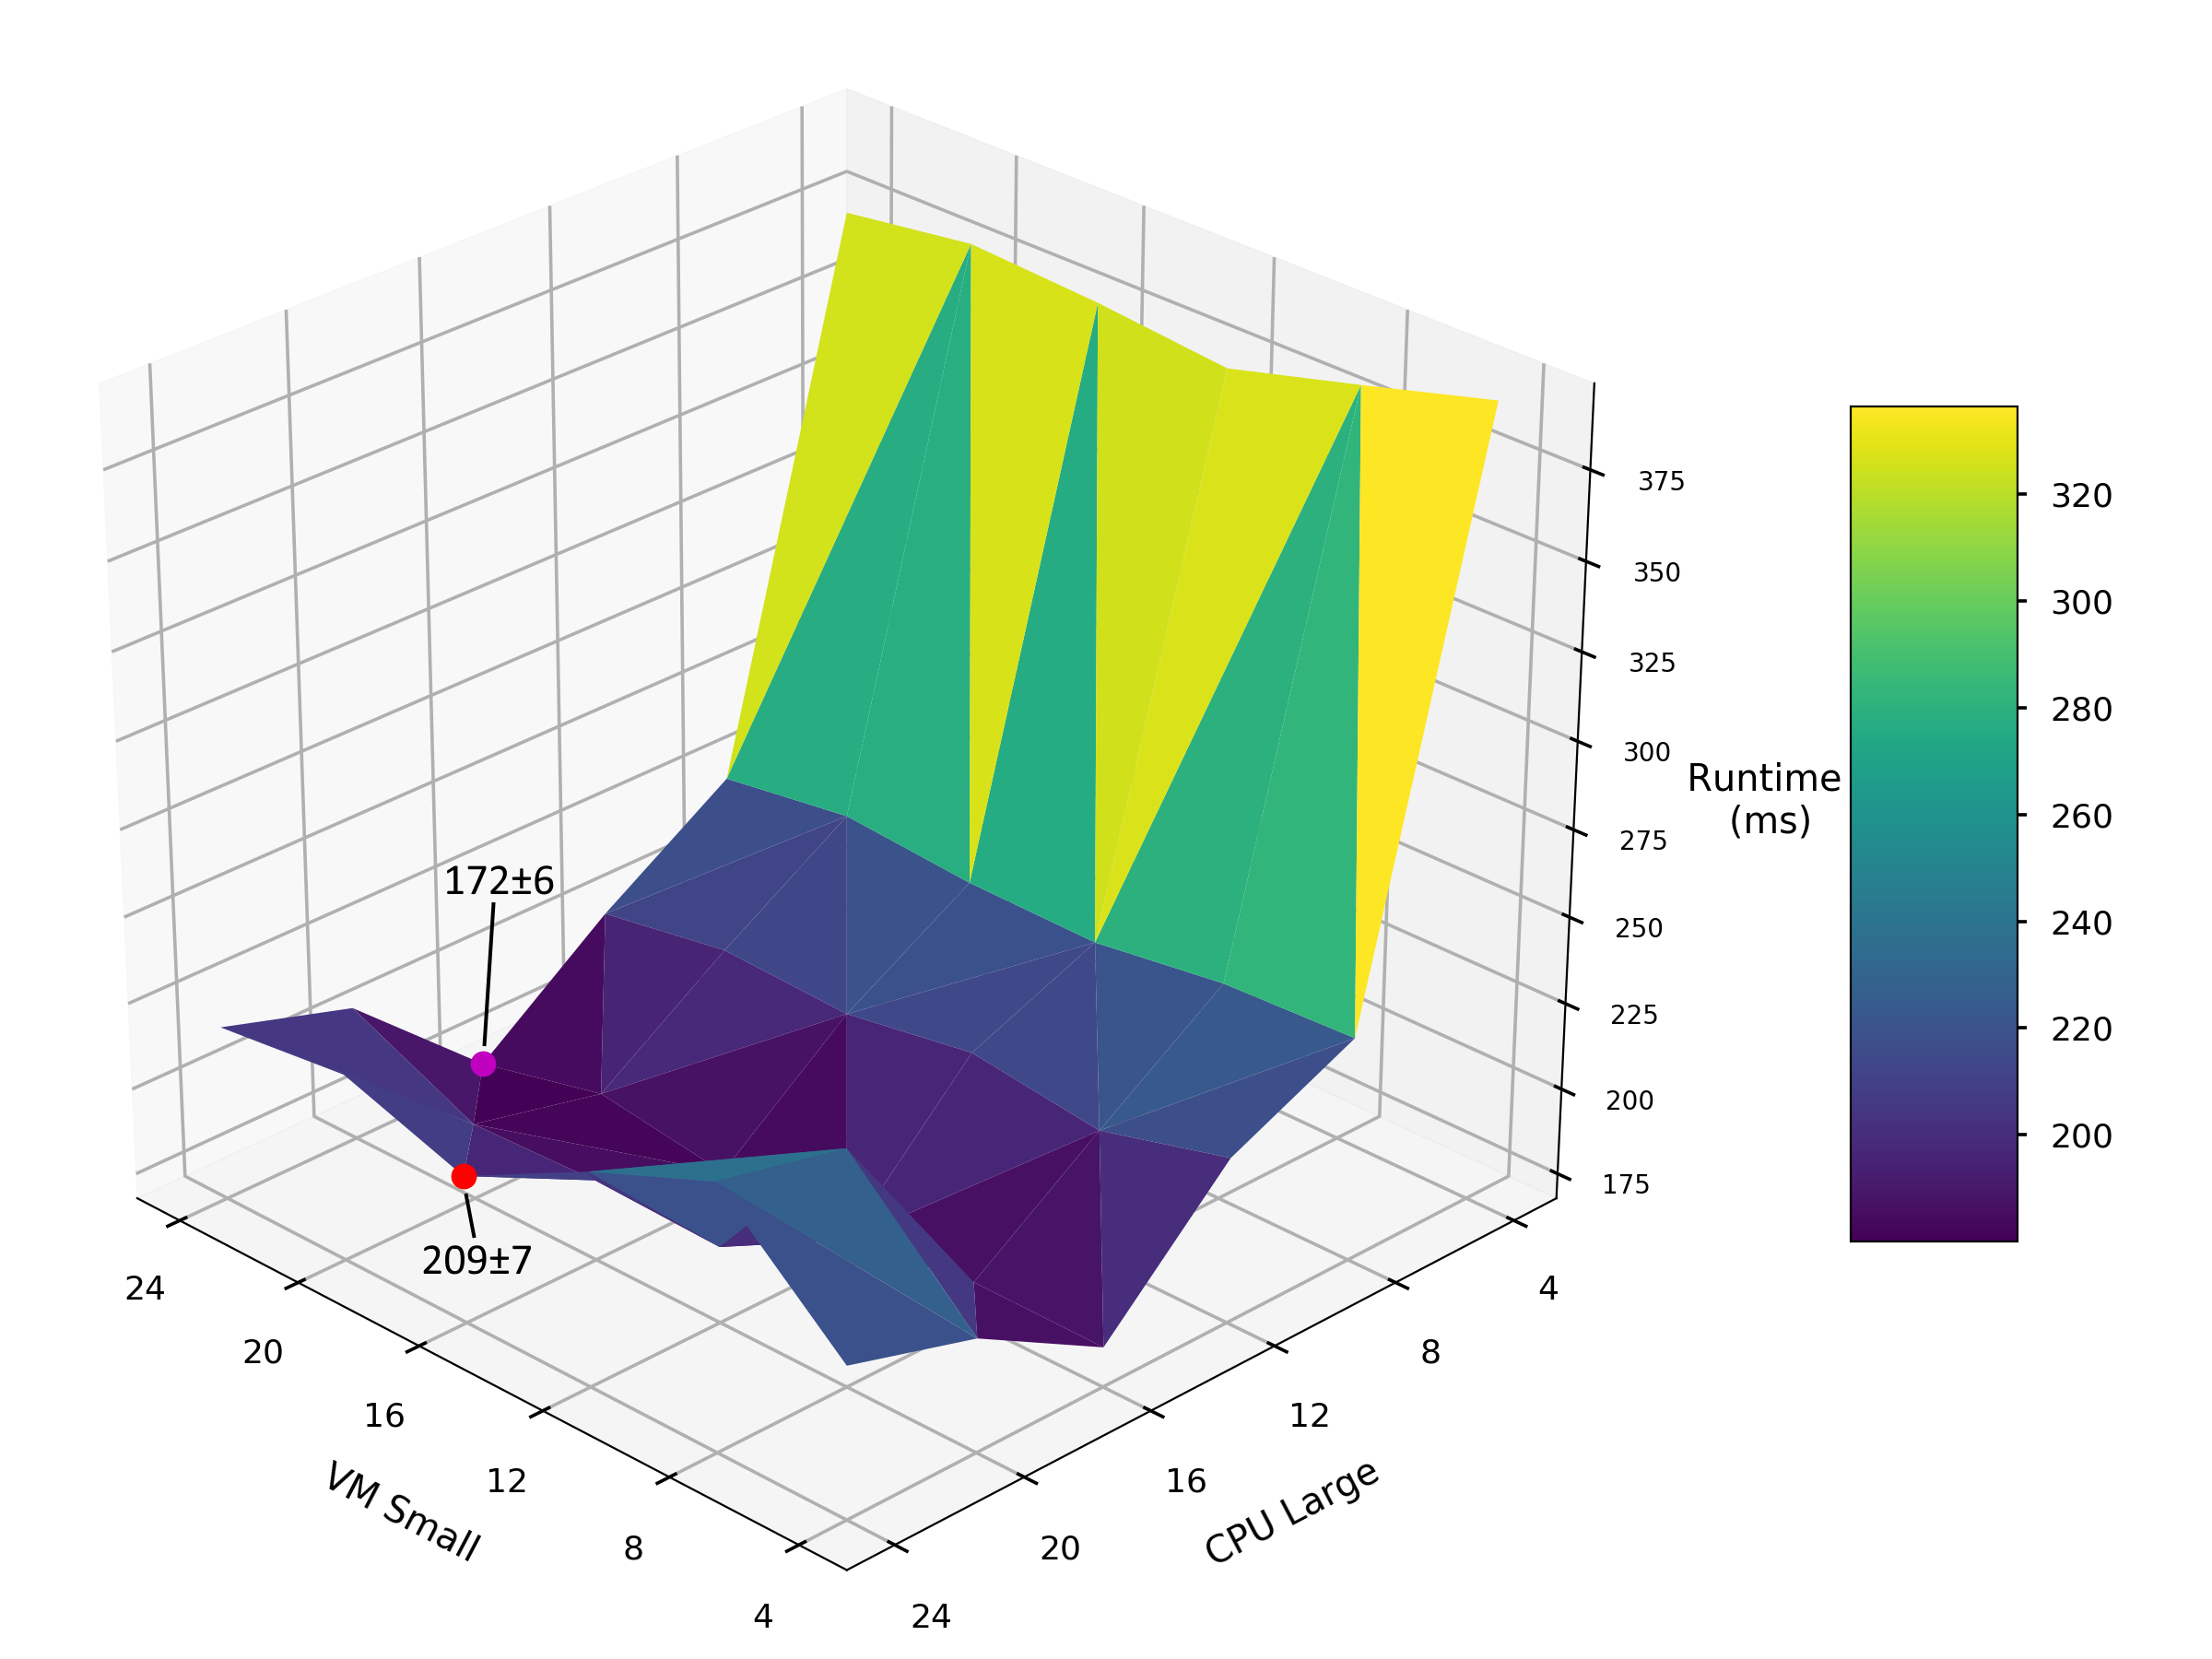
\includegraphics[width=1\textwidth]{graphics/contention/spa/otwc_vm_small_and_cpu_large.png}
    \caption{A 3D graph showing the total (summed) runtimes in milliseconds of the VM small and CPU large workloads running in contention on spa, and how they are affected by the number of workers assigned to each program. The red dot shows the result we would get if we used settings which were optimal when these programs were run in isolation. The purple dot shows the overall optimal case, which comparatively has a speedup of 1.22. This is what we could gain with a contention aware plastic parallel programming library. \\
    These results represent the case where the number of cores assigned to each program is optimal, (in this case, num cores for VM small = 24 and num cores for CPU large = 24.) Each point is the mean of 100 runs, with insignificant variance.}
    \label{fig:con_spa_vm_small_and_cpu_large}
\end{figure}



\subsection{Evaluating VM Small and VM Large in Contention}
\label{section:results:evaluating_vm_small_and_vm_large_in_contention}

The results presented in figure \ref{fig:con_spa_vm_small_and_vm_large} are contrary to what we might expect. The VM small and large workloads directly compete for the use of system resources, and as such, we would expect them to interfere with each other. However, these results do not reflect this. In fact, we see a speedup of merely 1.06. Looking back at our previous results, (in sections \ref{section:results:finding_the_optimal_thread_couonts_for_the_vm_small_workload} and \ref{section:results:finding_the_optimal_thread_couonts_for_the_vm_large_workload},) this is actually not wholly unexpected, as in all cases we saw evidence of the critical resource (in this case the virtual memory) becoming saturated. This would explain why we see this plateau in our graph, and in particular why significant changes to the assignments of threads does not significantly affect our performance, since the number of threads does not directly relate to the performance of a VM workload.

For our contention aware plastic parallel programming library, the takeaway here is that for applications where the virtual memory is a performance critical resource, we may not be able to attain performance gains where we would expect, or at all. As such, an optimal strategy in this situation would be to minimise the overall number of threads used, in order to minimise overhead and free up resources for other programs running on the system.



\begin{figure}[H]
    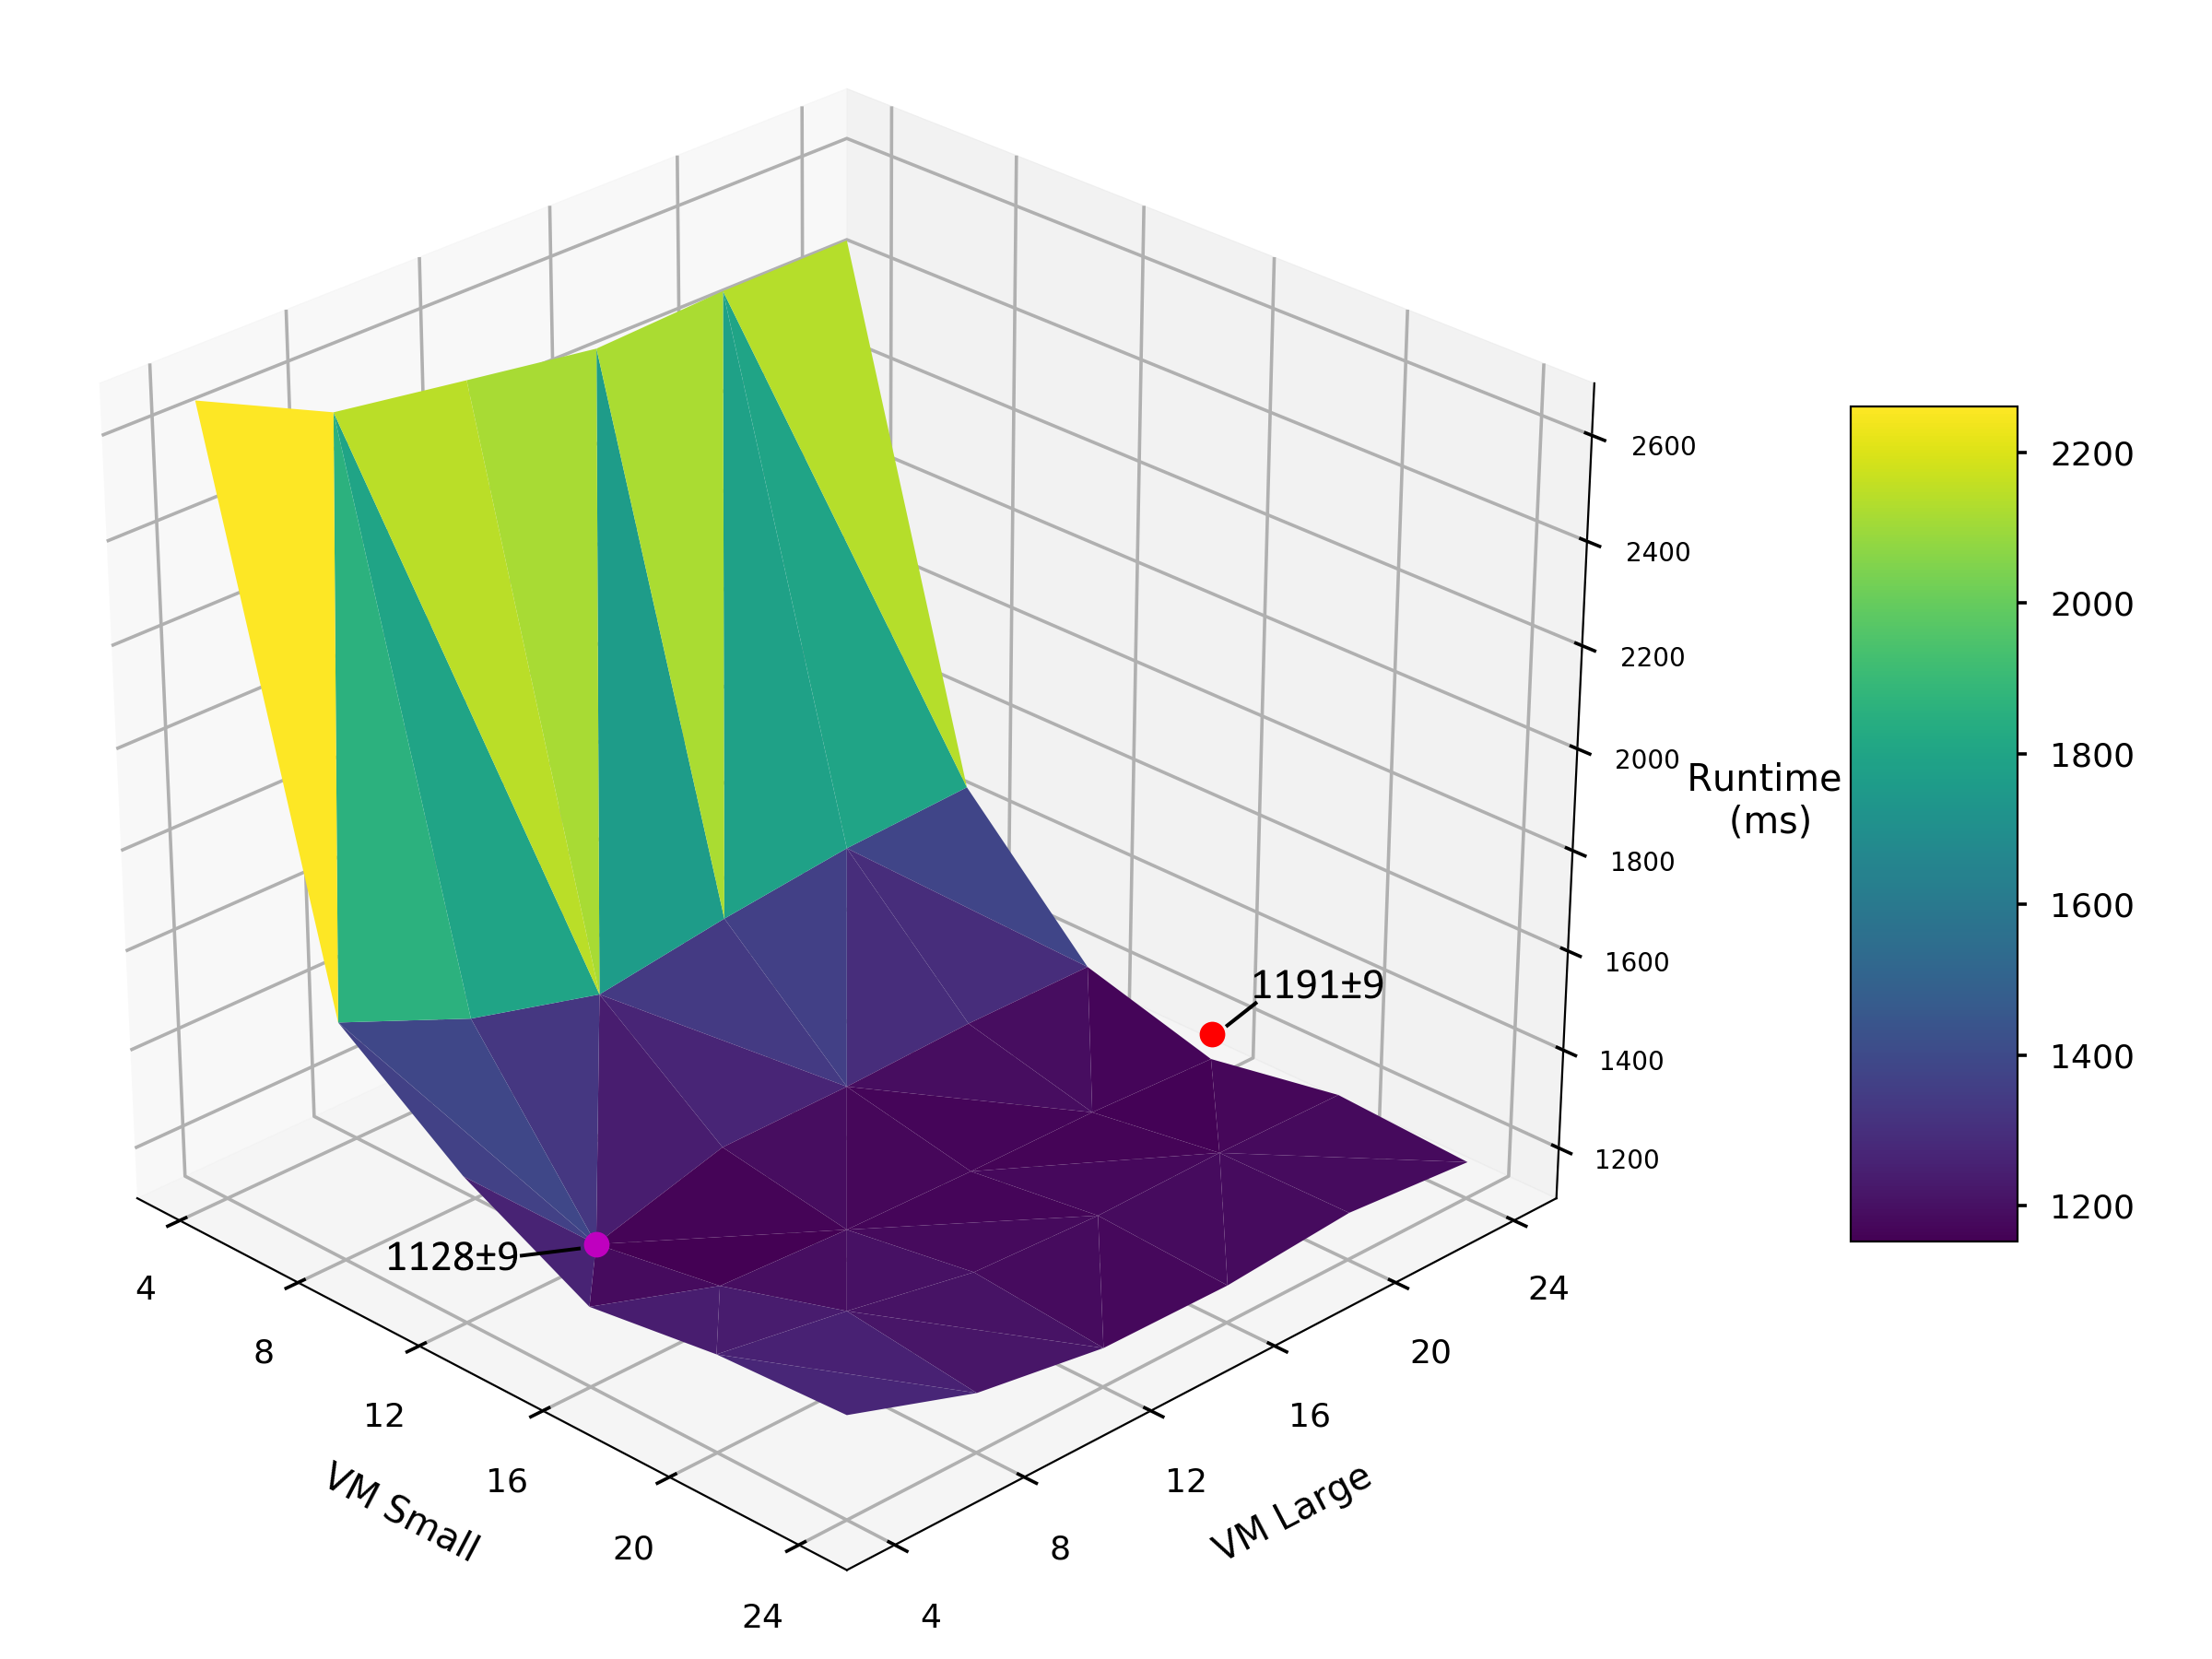
\includegraphics[width=1\textwidth]{graphics/contention/spa/otwc_vm_small_and_vm_large.png}
    \caption{A 3D graph showing the total (summed) runtimes in milliseconds of the VM small and VM large workloads running in contention on spa, and how they are affected by the number of workers assigned to each program. The red dot shows the result we would get if we used settings which were optimal when these programs were run in isolation. The purple dot shows the overall optimal case, which comparatively has a speedup of 1.06. This is what we could gain with a contention aware plastic parallel programming library. \\
    These results represent the case where the number of cores assigned to each program is optimal, (in this case, num cores for VM small = 16 and num cores for VM large = 24.) Each point is the mean of 100 runs, with insignificant variance.}
    \label{fig:con_spa_vm_small_and_vm_large}
\end{figure}



\subsection{Overall Conclusion}
\label{section:results:overall_conclusion2}

Again, the performance characteristics of our VM workloads show that their critical resource (the virtual memory) is saturated, as we saw when these programs were run in isolation (in section \ref{section:results:finding_optimal_thread_counts}.) This is best illustrated in figure \ref{fig:con_spa_vm_small_and_vm_large}.

These results have shown that there is clear potential for substantial speedups from the use of a contention aware plastic parallel programming library. We have seen that the performance characteristics of programs can change significantly when run in contention with others (particularly our ``small'' programs,) and that depending upon the situation, using parameters calculated from each program running in isolation may or may not be a good strategy.



\section{Additional Experiments}
\label{section:results:additional_experiments}

\subsection{Extended Contention Experiments}
\label{section:results:extended_contention_experiments}

The intention behind these extended contention experiments is to investigate a more complex scenario, involving three programs run in contention. To keep the total runtime of these experiments reasonable, we further restricted the range of each parameter in our tests compared to our previous contention experiments. We test 3 values per parameter, 4, 8, and 12, resulting in 729 tests per experiment. Testing 6 values per parameter would result in 46,656 tests!

This relatively low granularity means that there may exist an even better configuration of parameters that we simply did not evaluate. As such, this means that the overall speedup results that we see can only be improved upon. This goes for all of our experiments, as in each case, we had to sacrifice some detail due to time constraints, however this is especially applicable here, as we had to significantly restrict the number of combinations we tested.

The result presented in figure \ref{fig:spa_three_progs_results} shows the speedup of one combination of programs, run on spa. The results presented in figure \ref{fig:xxxii_three_progs_results} show the speedups of different combinations of programs, run on XXXII. Comparing the case with three instances of CPU small, we can see some interesting features. Notably, that the speedup we see on spa is much more drastic compared to the speedup on XXXII. Also, we see that whilst the independent runtime on spa is worse than either case on XXXII, the contention aware runtime is significantly better than either case on XXXII. Throughout our other tests, taking a look at our raw data, we observe that spa proved to be the faster machine, with anywhere up to a 1.8x speedup compared to the same workload on XXXII. We would therefore expect the contention aware runtime for spa to be an improvement over XXXII, and this suggests that the independent case for spa may simply a particularly bad configuration of parameters.

Looking at the other results from XXXII, presented in figure \ref{fig:xxxii_three_progs_results}, we can see another interesting feature. The situations involving purely CPU workloads experienced speedups from 1.13 to 1.18, whereas the situations involving VM workloads saw more significant speedups of 1.39 and 2.12, as well as much longer overall runtimes. This is intuitive, as memory operations are typically much more expensive compared to purely computational operations, and as such, using sub-optimal parameters for a memory dependent application may result in larger slowdowns compared to a CPU dependent application.



\begin{figure}[H]
    \centerline{
    \begin{tabular}{||c c c c c c c c c||} 
            \hline
            Kernel 1 & Size 1 & Kernel 2 & Size 2 & Kernel 3 & Size 3 & \multicolumn{1}{p{3cm}}{\centering Independent \\ Runtime} & \multicolumn{1}{p{3cm}}{\centering Contention Aware \\ Runtime} & Speedup \\ [0.5ex] 
            \hline\hline
            CPU & Small & CPU & Small & CPU & Small & $385\pm2$ ms & $159\pm6$ ms & 2.43 \\ [1ex] 
            \hline
        \end{tabular}
    }
    \caption{A table showing the total runtimes of different combinations of three programs in milliseconds run on spa, first using settings as if they were individually profiled (Independent Runtime,) then using contention aware settings (Contention Aware Runtime,) and the speedup between them. Due to the high dimensionality of each case, we present this as a table, rather than a sequence of graphs. Each data point is the mean of 100 runs, shown with 95\% confidence intervals.}
    \label{fig:spa_three_progs_results}
\end{figure}






\begin{figure}[H]
    \centerline{
    \begin{tabular}{||c c c c c c c c c||} 
            \hline
            Kernel 1 & Size 1 & Kernel 2 & Size 2 & Kernel 3 & Size 3 & \multicolumn{1}{p{3cm}}{\centering Independent \\ Runtime} & \multicolumn{1}{p{3cm}}{\centering Contention Aware \\ Runtime} & Speedup \\ [0.5ex] 
            \hline\hline
            CPU & Small & CPU & Small & CPU & Small & $298\pm7$ ms & $251\pm12$ ms & 1.18 \\
            \hline
            CPU & Small & CPU & Small & CPU & Large & $271\pm5$ ms & $236\pm13$ ms & 1.14 \\ 
            \hline
            CPU & Small & CPU & Small & VM & Small & $1144\pm28$ ms & $826\pm14$ ms & 1.39 \\ 
            \hline
            CPU & Small & CPU & Small & VM & Large & $3390\pm57$ ms & $1602\pm54$ ms & 2.12 \\ 
            \hline
            CPU & Small & CPU & Large & CPU & Large & $236\pm5$ ms & $209\pm3$ ms & 1.13 \\ [1ex]
            \hline
        \end{tabular}
    }
    \caption{A table showing the total runtimes of different combinations of three programs in milliseconds run on XXXII, first using settings as if they were individually profiled (Independent Runtime,) then using contention aware settings (Contention Aware Runtime,) and the speedup between them. Due to the high dimensionality of each case, we present this as a table, rather than a sequence of graphs. Each data point is the mean of 100 runs, shown with 95\% confidence intervals.}
    \label{fig:xxxii_three_progs_results}
\end{figure}